\documentclass{article} % loại tài liệu
\usepackage[utf8]{vietnam} % tiếng Việt
\usepackage[left = 3.5cm,right = 2cm,top = 3.5cm,bottom = 3cm]{geometry} % căn lề
\usepackage{tikz} % vẽ hình
\usetikzlibrary{calc} % tính toán vẽ hình
\usepackage{graphicx} % hình ảnh
\usepackage{pdfpages} % thêm file pdf bao_cao_tien_do

% Sử dụng gói color để thay đổi màu
\usepackage{color} %* mau_sac
% Sử dụng gói xcolor để mở rộng tính năng thay đổi màu
\usepackage{xcolor} %* mau_sac
% \definecolor{HustRed}{RGB}{206,22,40}
% \definecolor{HustYellow}{RGB}{242,193,8}
\definecolor{BackgroundCode}{RGB}{242,242,235}

% Sử dụng gói caption để tùy chỉnh caption
\usepackage{caption}%* caption
% Sử dụng gói listing để hiển thị mã nguồn
\usepackage{listing}
% \renewcommand*{\listlistingname}{Danh sách mã nguồn}
\DeclareCaptionLabelFormat{code_caption}{{Mã nguồn #2}}
\captionsetup*[listing]{labelformat = code_caption}

% Sử dụng gói minted để đính kèm và định dạng mã nguồn
\usepackage{minted} %! code_python
\setminted{
fontsize = \footnotesize, % Cỡ chữ cho mã nguồn
frame = lines, % Hiển thị đường viền xung quanh mã nguồn
framesep = 2mm, % Khoảng cách giữa đường viền và nội dung mã nguồn
bgcolor = BackgroundCode, % Màu nền cho mã nguồn
linenos, % Hiển thị số dòng ở bên trái
autogobble, % Tự động loại bỏ khoảng trắng ở đầu mỗi dòng
}

\begin{document} % bắt đầu
%%%%%%%%%%%%%%%%%%%%%%%%%%%%%%%%%%%%%
% \begin{titlepage}
\begin{tikzpicture}[remember picture, overlay]
\draw [line width = 3pt]
($ (current page.north west) + (3.0cm, - 2.5cm)$)
rectangle
($ (current page.south east) + (- 2.5cm, 2.5cm)$);
\draw [line width = 0.5pt]
($ (current page.north west) + (3.1cm, - 2.6cm)$)
rectangle
($ (current page.south east) + (- 2.6cm, 2.6cm)$);
\end{tikzpicture}
\begin{center}
\vspace{- 0.4cm}
\textbf{ĐẠI HỌC BÁCH KHOA HÀ NỘI} \\
\textbf{VIỆN TOÁN ỨNG DỤNG VÀ TIN HỌC} \\
\textbf{******}
\vspace{0.8cm}

\begin{figure}[h]
\centering

\includegraphics[scale = .5]{pictures/logoBK.png}
\end{figure}
\vspace{0.7cm}
\textbf{\fontsize{16pt}{30pt}\selectfont {BÁO CÁO ĐỒ ÁN II}} \\
\vspace{1cm}
\textbf{\fontsize{20pt}{24pt}\selectfont {ĐỀ TÀI:}} \\
\textbf{\fontsize{19pt}{24pt}\selectfont {Xây dựng kiến trúc vi dịch vụ cho bài toán hóa đơn điện tử}} \\
% \textbf{\fontsize{20pt}{24pt}\selectfont {Sử dụng thiết kế hướng miền xây dựng kiến trúc vi dịch vụ cho bài toán hóa đơn điện tử}} \\
\end{center}
\vspace{0.7cm}

\hspace{2.4cm}
\begin{minipage}{0.8\textwidth}
\textbf{Giảng viên hướng dẫn: TS. Vũ Thành Nam}
\end{minipage}

\hspace{3cm}
\begin{minipage}{0.7\textwidth}
\begin{tabular}{l l l}
Sinh viên thực hiện & Vũ Văn Nghĩa \\
Mã số sinh viên & 20206205 \\
Lớp & Toán Tin 02 - K65 \\
\end{tabular}
\end{minipage}

\hspace{2.4cm}
\begin{center}
\textbf{\fontsize{20pt}{24pt}\selectfont {Chuyên ngành: Toán Tin}}
\end{center}

\vspace{0.5cm}
\begin{center}
\textbf{Hà Nội, \the\month - \the\year}
\end{center}
\end{titlepage}

% % Trang trắng không có nội dung và không có số trang
\pagestyle{empty}
\thispagestyle{empty}

\mbox{} % Một hộp rỗng để trang không bị trắng toàn bộ

% \newpage

\begin{center}
{\bfseries NHẬN XÉT CỦA GIẢNG VIÊN HƯỚNG DẪN}
\end{center}

\begin{enumerate}
\item Mục đích và nội dung của đồ án:
\vspace{20ex} % Thêm khoảng cách dọc
\item 	Kết quả đạt được:
\vspace{20ex} % Thêm khoảng cách dọc
\item 	Ý thức làm việc của sinh viên:
\vspace{20ex} % Thêm khoảng cách dọc
\end{enumerate}

\hspace{0.4\textwidth}
\begin{minipage}{0.5\textwidth}
\noindent\begin{center}
\textit{Hà Nội, \today} \\
\textbf{Giảng viên hướng dẫn} \\
\textit{(Ký và ghi rõ họ tên)}
\end{center}
\end{minipage}

\pagestyle{empty}

\newpage

% 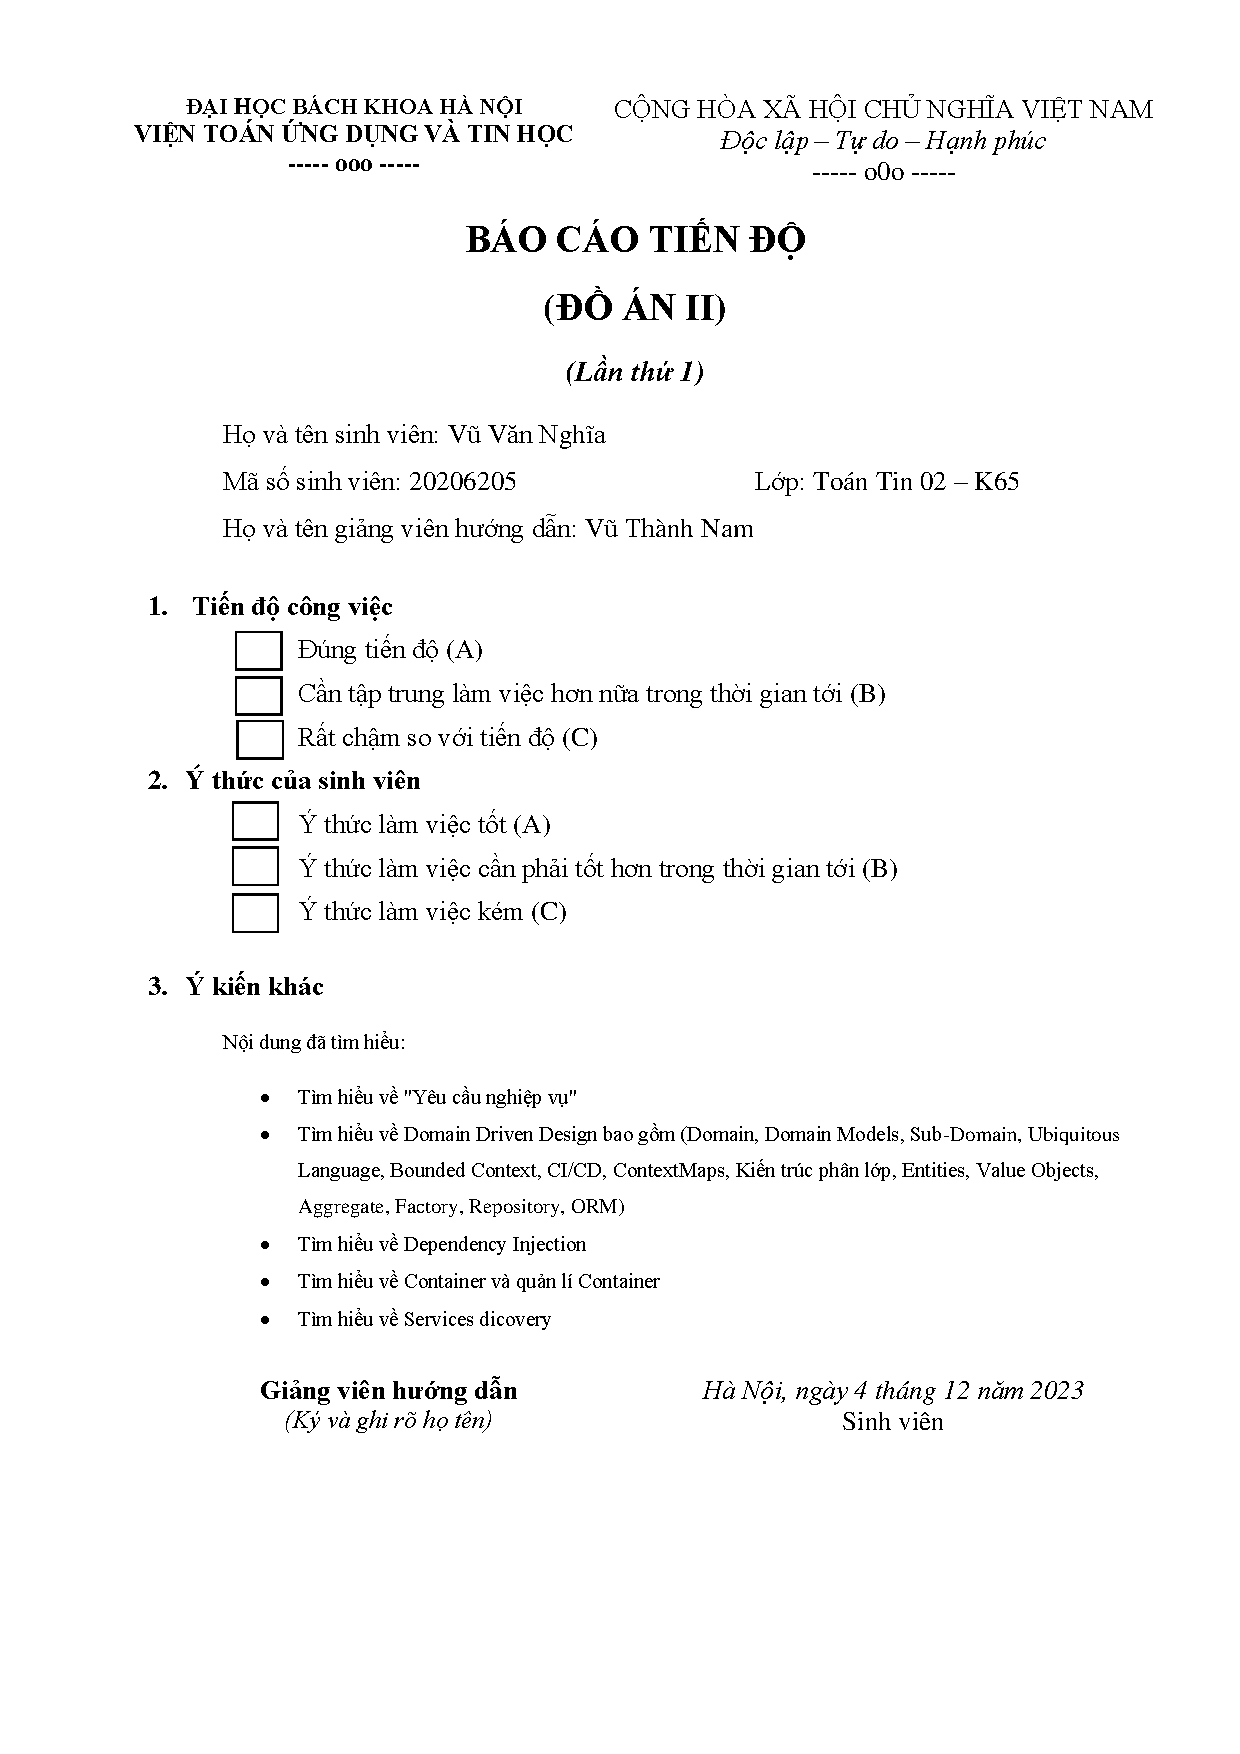
\includepdf[pages = -]{contents/bao_cao_tien_do_1.pdf}
% 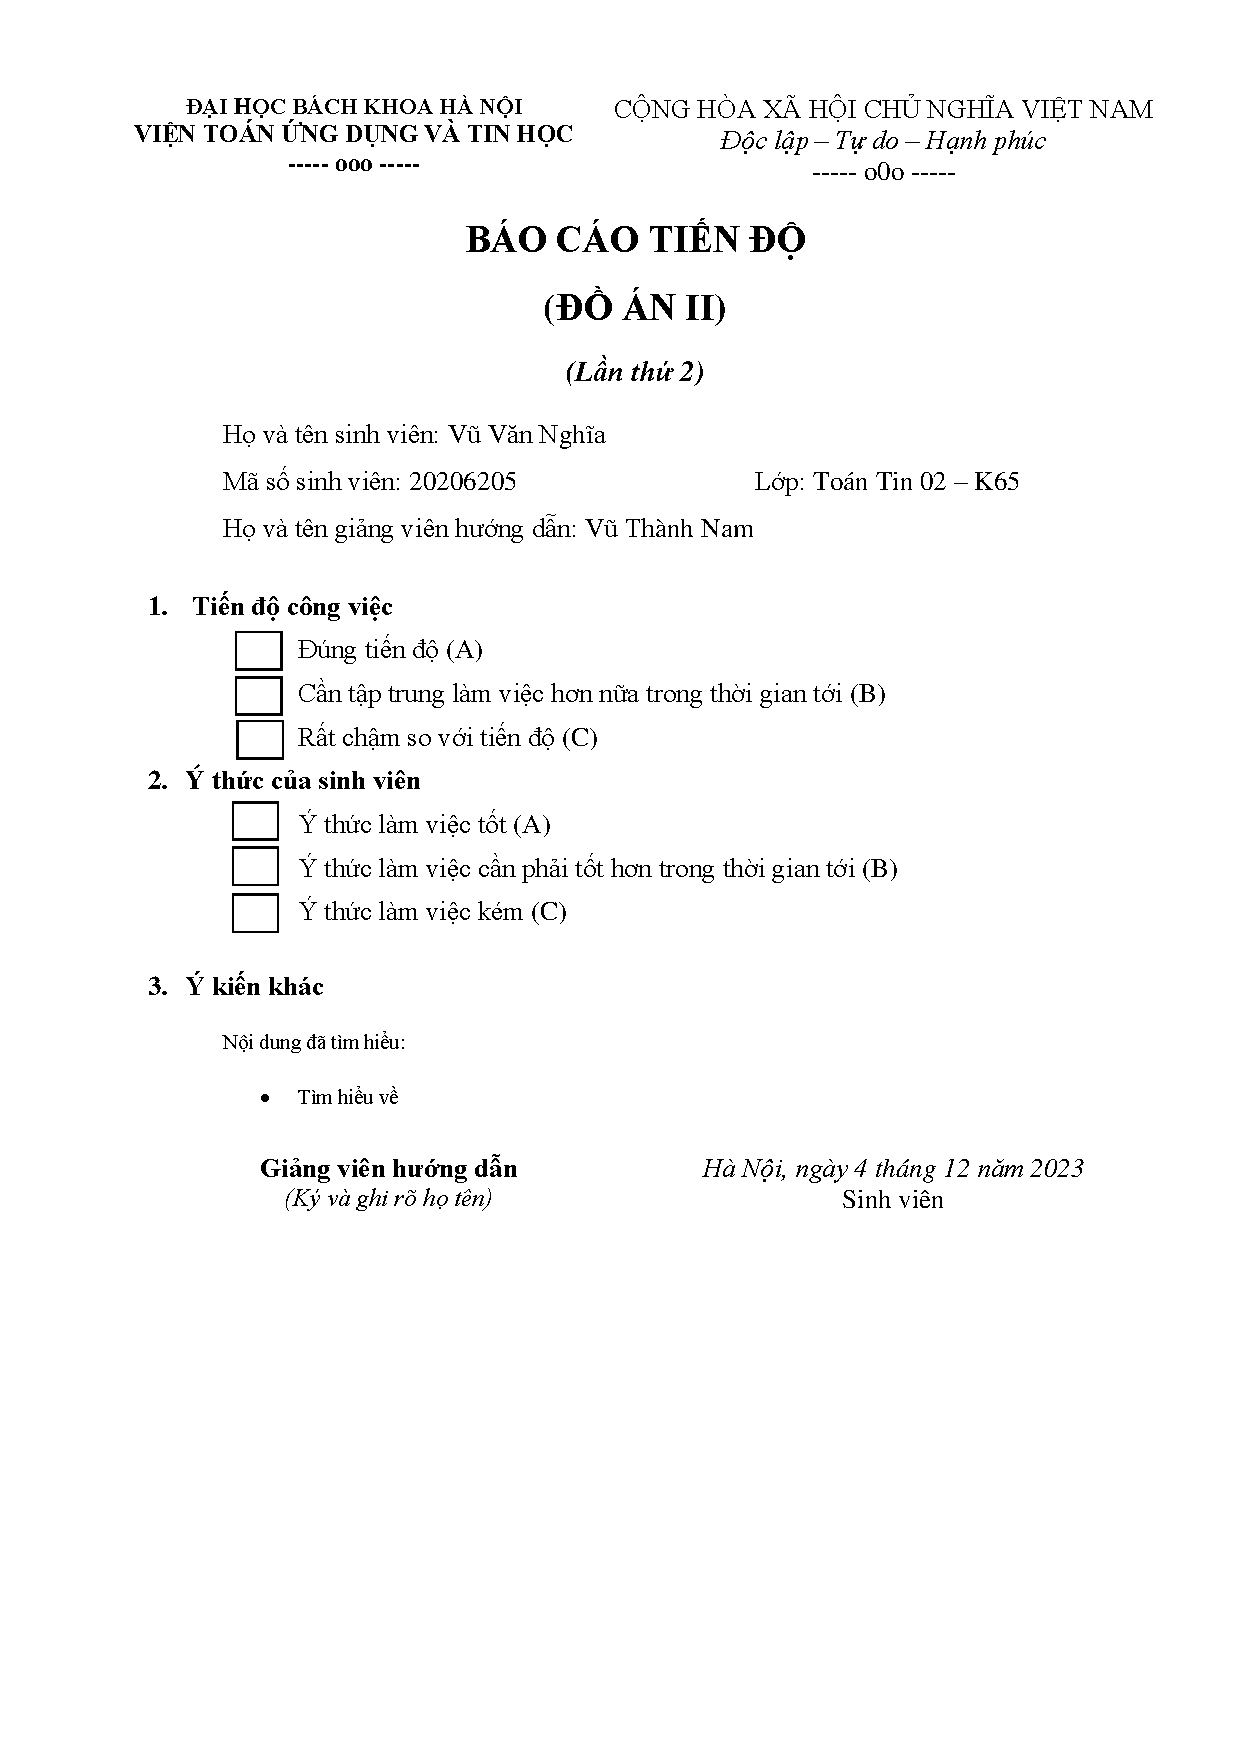
\includepdf[pages = -]{contents/bao_cao_tien_do_2.pdf}

% \newpage
\renewcommand*\contentsname{\centering MỤC LỤC}
\tableofcontents
\newpage


% \newpage

\section*{\centering LỜI CẢM ƠN}

\addcontentsline{toc}{section}{LỜI CẢM ƠN}

\newpage


% \newpage

\section*{\centering LỜI MỞ ĐẦU}

\addcontentsline{toc}{section}{LỜI MỞ ĐẦU}

\newpage
% \newpage
\section*{\centering TÓM TẮT NỘI DUNG ĐỒ ÁN}
\addcontentsline{toc}{section}{TÓM TẮT NỘI DUNG ĐỒ ÁN}
\newpage
% \newpage
\section*{\centering ĐÁNH GIÁ VÀ THẢO LUẬN}
\addcontentsline{toc}{section}{ĐÁNH GIÁ VÀ THẢO LUẬN}
\newpage

% \newpage
\section*{\centering DANH SÁCH BẢNG}
\addcontentsline{toc}{section}{DANH SÁCH BẢNG}
\makeatletter
\renewcommand\listoftables{            
\@starttoc{lot}            
}
\makeatother 
\listoftables  
\newpage
% \newpage
\section*{\centering DANH SÁCH HÌNH ẢNH}
\addcontentsline{toc}{section}{DANH SÁCH HÌNH ẢNH}
\makeatletter
\renewcommand\listoffigures{      
\@starttoc{lof}      
}
\makeatother
\listoffigures  
\newpage
% \newpage

\section*{\centering DANH SÁCH MÃ NGUỒN}

\addcontentsline{toc}{section}{DANH SÁCH MÃ NGUỒN}

\makeatletter

\renewcommand\listoflistings{

\@starttoc{lol}

}

\makeatother

\listoflistings

\newpage
% \newpage
\section*{\centering DANH SÁCH CÁC CỤM TỪ VIẾT TẮT}
\addcontentsline{toc}{section}{DANH SÁCH CÁC CỤM TỪ VIẾT TẮT}

% @sau

\begin{table}[h]
\centering
\begin{tabular}{|c|c|c|c|}
\hline
STT & Từ viết tắt & Từ viết đầy đủ & Mô tả \\
\hline
Dong1 & Dong1 & Cot1 & Cot2 \\
\hline
Dong2 & Dong2 & Cot1 & Cot2 \\
\hline
\end{tabular}
\caption{ViDuBangThuong}
\end{table}

\newpage

% API; Application Programming Interface; Giao diện lập trình ứng dụng
% CI/CD; Continuous Integration (CI) and Continuous Delivery (CD) ; Quá trình tích hợp và chuyển giao liên tục
% thiết kế hướng miền ; thiết kế hướng miền; Kỹ thuật thiết kế theo hướng miền
% DI; Dependency Injection; Cơ chế tiêm sự phụ thuộc giữa các đối tượng
% HTTP; Hypertext Transfer Protocol; Giao thức truyền tải siêu văn bản
% JSON; JavaScript Object Notation; Một kiểu dữ liệu mở rộng của JavaScript
% ORM; Object Relational Mapping; Một kỹ thuật ánh xạ các đối tượng lập trình với từng bảng trong CSDL quan hệ
% Cơ sở dữ liệu ; CSDL ;
% Tạo (Create), Đọc (Read), Sửa (Update), Xóa (Delete) ; CRUD ;
% Kubernetes ; K8s ; kubernetes
% Số điện thoại ; SĐT ;
% UML
% MVC; Model View Controller; Một mẫu thiết kế ứng dụng
% SQL

SOA; Service Oriented Architecture; Kiến trúc hướng dịch vụ
SOAP; Simple Object Access Protocol; Một giao thức để truy cập dịch vụ web
SPA; Single Page Application; Kiểu ứng dụng một trang
REST; Representational State Transfer; Một tiêu chuẩn thiết kế các API sử dụng cho các dịch vụ web
URL; Uniform Resource Locator ; Địa chỉ định vị tài nguyên trên Internet
XML; Extensible Markup Language; Ngôn ngữ đánh dấu mở rộng

% TCT ; TCT ;
Người nộp thuế ; NNT ;
Mã số thuế ; MST ;
Hóa đơn điện tử ; HĐĐT ;
Cơ quan thuế ; CQT ;
Công nghệ thông tin ; CNTT ;


% % STT; Tiếng Anh; Tiếng Việt
% @sau

% kiến trúc nguyên khối, kiến trúc nguyên khối
% kiến trúc nguyên khối, kiến trúc nguyên khối
% kiến trúc vi dịch, kiến trúc vi dịch
% kiến trúc vi dịch, kiến trúc vi dịch
% kiến trúc vi dịch, kiến trúc vi dịch
% kiến trúc vi dịch, kiến trúc vi dịch
% thiết kế hướng miền, thiết kế hướng miền
% thiết kế hướng miền, thiết kế hướng miền

1 thiết kế hướng miền
Thiết kế hướng lĩnh vực
2 Domain (không dịch)
3 Abstraction Trừu tượng
4 chuyên gia ngành

%%%%%%%%%%%
\section{Giới thiệu}

Trong thời đại ngày nay, nhu cầu phát triển ứng dụng và hệ thống ngày càng tăng, đặt ra thách thức đối với kiến trúc phần mềm. Kiến trúc nguyên khối đã phục vụ hiệu quả trong quá khứ, nhưng kiến trúc này bắt đầu gặp khó khăn đối mặt với sự phức tạp, khả năng mở rộng và khả năng đáp ứng linh hoạt với thay đổi nhanh chóng trong yêu cầu kinh doanh.

Kiến trúc vi dịch vụ là giải pháp cho những thách thức trên. Kiến trúc vi dịch vụ chia dự án thành những dịch vụ nhỏ độc lập, mỗi dịch vụ chịu trách nhiệm về một chức năng cụ thể. Từ đó, giảm sự phức tạp của dự án tăng tính linh hoạt và dễ dàng quản lý.

Việc vận dụng kết hợp giữa kiến trúc vi dịch vụ và thiết kế hướng miền là một cách tiếp cận toàn diện, giúp xác định và tổ chức các dịch vụ dựa trên việc hiểu rõ về lĩnh vực kinh doanh. Thiết kế hướng miền xây dựng mô hình dựa trên yêu cầu nghiệp vụ thực tế, từ đó dự án phản ánh đúng các quy trình kinh doanh.

\subsection{Giới thiệu về bài toán hóa đơn điện tử}

Bài toán hóa đơn điện tử là một phần quan trọng của quá trình chuyển đổi số. Trong quá khứ, mọi người thường sử dụng hóa đơn giấy truyền thống. Ngày nay, khi có quy định kế toán và quản lý tài chính, hóa đơn điện tử đã trở nên phổ biến giúp giảm bớt sự phụ thuộc vào giấy tờ. Cùng với sự phát triển của khoa học công nghệ đã giúp quản lí hiệu quả công việc và tối ưu hóa quy trình kế toán và tài chính.

Theo em tìm hiểu có các khái niệm và căn cứ pháp lý liên quan sau đây:

\subsubsection{Hóa đơn}

%%%%%%%%%%%%%%%%%%%%%%%%%%%%%%%%%%%%%!

Hóa đơn là chứng từ kế toán do tổ chức, cá nhân bán hàng hóa, cung cấp dịch vụ lập, ghi nhận thông tin bán hàng hóa, cung cấp dịch vụ. Hóa đơn được thể hiện theo hình thức hóa đơn điện tử hoặc hóa đơn do cơ quan thuế đặt in.

%%%%%%%%%%%%%%%%%%%%%%%%%%%%%%%%%%%%%!



\subsubsection{Hóa đơn điện tử}

Hóa đơn điện tử là hóa đơn có mã hoặc không có mã của cơ quan thuế được thể hiện ở dạng dữ liệu điện tử do tổ chức, cá nhân bán hàng hóa, cung cấp dịch vụ lập bằng phương tiện điện tử để ghi nhận thông tin bán hàng hóa, cung cấp dịch vụ theo quy định của pháp luật về kế toán, pháp luật về thuế, bao gồm cả trường hợp hóa đơn được khởi tạo từ máy tính tiền có kết nối chuyển dữ liệu điện tử với cơ quan thuế, trong đó:

a. Hóa đơn điện tử có mã của cơ quan thuế là hóa đơn điện tử được cơ quan thuế cấp mã trước khi tổ chức, cá nhân bán hàng hóa, cung cấp dịch vụ gửi cho người mua. Mã của cơ quan thuế trên hóa đơn điện tử bao gồm số giao dịch là một dãy số duy nhất do hệ thống của cơ quan thuế tạo ra và một chuỗi ký tự được cơ quan thuế mã hóa dựa trên thông tin của người bán lập trên hóa đơn.

b. Hóa đơn điện tử không có mã của cơ quan thuế là hóa đơn điện tử do tổ chức bán hàng hóa, cung cấp dịch vụ gửi cho người mua không có mã của cơ quan thuế.

% \subsubsection{Bắt buộc sử dụng hóa đơn điện tử từ 01/07/2022}
% Nghị định này có hiệu lực thi hành kể từ ngày 01 tháng 7 năm 2022, khuyến khích cơ quan, tổ chức, cá nhân đáp ứng điều kiện về hạ tầng công nghệ thông tin áp dụng quy định về hóa đơn, chứng từ điện tử của Nghị định này trước ngày 01 tháng 7 năm 2022.

% Chủ đề

Theo quy định, tất cả các doanh nghiệp, tổ chức và hộ kinh doanh đều bắt buộc phải chuyển từ sử dụng hóa đơn giấy sang hóa đơn điện tử bắt đầu từ tháng 07/2022. Vì vậy, nhu cầu sử dụng và xử lý hóa đơn điện tử trở nên rất lớn. Do đó ở đồ án này, em chọn chủ đề về quản lý hóa đơn điện tử.

% \subsubsection{Bản thể hiện của hóa đơn điện tử}
% \input{contents/ban_the_hien_cua_hoa_don_dien_tu}

% \subsubsection{Lưu trữ hóa đơn điện tử}
% Thời gian?
% 
 
\textbf{Theo quy định tại khoản 1 Điều 11 Thông tư 32/2011/TT-BTC:} 




 
  

  Người bán, người mua hàng hoá, dịch vụ sử dụng hóa đơn điện tử để ghi sổ kế toán, lập báo cáo tài chính phải lưu trữ hóa đơn điện tử theo thời hạn quy định của Luật Kế toán. Trường hợp hóa đơn điện tử được khởi tạo từ hệ thống của tổ chức trung gian cung cấp giải pháp hóa đơn điện tử thì tổ chức trung gian này cũng phải thực hiện lưu trữ hóa đơn điện tử theo thời hạn nêu trên.
  
\textbf{Theo quy định tại khoản 5 Điều 41 Luật số 88/2015/QH13:} 

  
  1. Tài liệu kế toán phải được lưu trữ theo thời hạn sau đây:
  
  a. Ít nhất là 05 năm đối với tài liệu kế toán dùng cho quản lý, điều hành của đơn vị kế toán, gồm cả chứng từ kế toán không sử dụng trực tiếp để ghi sổ kế toán và lập báo cáo tài chính.
  
  b. Ít nhất là 10 năm đối với chứng từ kế toán sử dụng trực tiếp để ghi sổ kế toán và lập báo cáo tài chính, sổ kế toán và báo cáo tài chính năm, trừ trường hợp pháp luật có quy định khác.
  
  c. Lưu trữ vĩnh viễn đối với tài liệu kế toán có tính sử liệu, có ý nghĩa quan trọng về kinh tế, an ninh, quốc phòng.
  
  => Như vậy, hóa đơn điện tử dạng tệp XML sẽ được lưu trữ trên hệ thống hóa đơn điện tử của nhà cung cấp hoặc doanh nghiệp có thể tải về để tự lưu trữ. Thời gian lưu trữ là 10 năm theo quy định của pháp luật.
  

% \subsubsection{Một số lợi ích của hóa đơn điện tử}
% Giúp tiết kiệm chi phí in ấn, lưu trữ và bảo quản.
Loại bỏ rủi ro cháy, hỏng hoặc mất và dễ dàng sao lưu.
Dễ dàng linh hoạt trong việc tra cứu, phát hành, quản lý và tạo báo cáo.
Tối ưu hóa quá trình kế toán (giảm sai sót và tiết kiệm thời gian) và giảm thủ tục giấy tờ.
Theo dõi tình hình tài chính của công ty (doanh thu, chi phí, lợi nhuận).
Tuân thủ các quy định về thuế và pháp luật.
Thể hiện tính minh bạch trong quá trình kinh doanh (bảo vệ quyền lợi của cả người mua và người bán).

% \subsection{Giới thiệu về kiến trúc vi dịch vụ}
% \subsubsection{Kiến trúc nguyên khối}
% Trước khi kiến trúc vi dịch vụ trở nên phổ biến, kiến trúc nguyên khối đã được áp dụng rộng rãi trong kiến trúc phần mềm truyền thống. Kiến trúc nguyên khối là kiến trúc phần mềm trong đó  tất cả các thành phần      của  dự án    được xây dựng thành một đơn vị triển khai    duy nhất. 

% Trong kiến trúc nguyên khối, bất kỳ thay đổi nào đối với một thành phần     đều yêu cầu toàn bộ ứng dụng phải được     kiểm thử   và triển khai lại. 




Điều này có thể dẫn đến chu kỳ phát triển và triển khai chậm hơn cũng như thiếu khả năng mở rộng vì ứng dụng có thể không đáp ứng được nhu cầu về chức năng hoặc lưu lượng truy cập ngày càng tăng. Tuy nhiên, kiến trúc nguyên khối thường thiết kế, phát triển và bảo trì đơn giản hơn so với các kiến trúc phân tán, khiến chúng trở thành lựa chọn phổ biến cho các ứng dụng quy mô nhỏ hơn hoặc các nhóm có nguồn lực hạn chế.


% 
Ví dụ: Mô hình MVC (Model - View - Controller) là một trong những dạng của kiến trúc nguyên khối.

Trong mô hình này, ứng dụng được chia thành ba thành phần chính:

Mô hình (Model): Đại diện cho dữ liệu và logic xử lý dữ liệu.

Giao diện (View): Đại diện cho giao diện người dùng.

Bộ điều khiển (Controller): Nhận yêu cầu người dùng thông qua View, sau đó tương tác với Model để làm việc với dữ liệu.

%  
 
 
 




\subsubsection{xxxxxxx}
% \newpage
\begin{center}
{\bfseries NHẬN XÉT CỦA GIẢNG VIÊN HƯỚNG DẪN}
\end{center}
1.	Mục đích và nội dung của đồ án:

\vspace{4ex} % Thêm khoảng cách dọc

2.	Kết quả đạt được:

3.	Ý thức làm việc của sinh viên:

Hà Nội, \today

\textbf{Giảng viên hướng dẫn}

\textit{(Ký và ghi rõ họ tên)}

\newpage

\end{document} % kết thúc

% \subsubsection{Kiến trúc vi dịch vụ}
% Kiến trúc vi dịch vụ chia dự án thành các thành phần nhỏ hơn được gọi là các dịch vụ.

Mỗi dịch vụ tập trung vào một khả năng kinh doanh cụ thể.

Các dịch vụ độc lập và giao tiếp với nhau thông qua hạ tầng mạng.

%

\end{document}

% và có thể được triển khai, mở rộng quy mô và duy trì độc lập với các dịch vụ khác trong hệ thống.

% Các dịch vụ độc lập về ngôn ngữ lập trình, CSDL, triển khai,...

% Các dịch vụ tương tác với nhau qua hạ tầng mạng.

% \begin{figure}[h]

% \centering

% 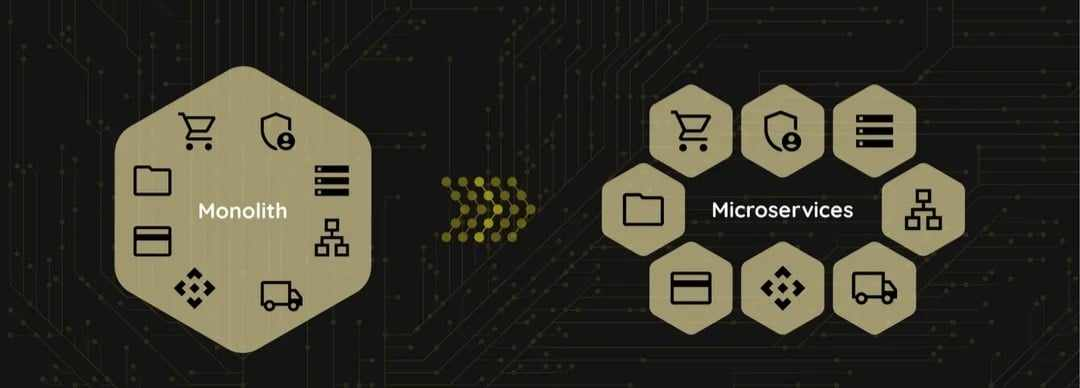
\includegraphics[height = 3cm]{pictures/ChuyenTu_KienTrucNguyenKhoi_Sang_KienTrucViDichVu.jpg}

% % \caption{ViDuHinhAnhTheoChieuDoc}

% \end{figure}

% \begin{figure}[h]

% \centering

% 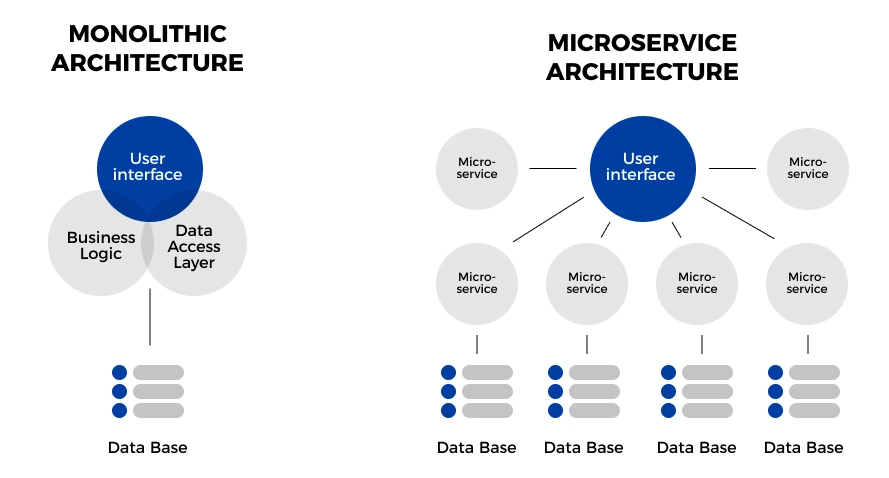
\includegraphics[height = 3cm]{pictures/AnhKhacNhau_KienTrucNguyenKhoi_KienTrucViDichVu.png}

% % \caption{ViDuHinhAnhTheoChieuDoc}

% \end{figure}

% Strangler Fig là chuyển mono sang dịch vụ



% \subsubsection{Một số đặc điểm và ưu điểm của kiến trúc vi dịch vụ}
% Kiến trúc vi dịch vụ có nhiều ưu điểm, đặc biệt với các dự án có quy mô lớn và phức tạp.

\begin{itemize}

    \item Kiến trúc vi dịch vụ phân chia dự án thành các dịch vụ nhỏ.

          \begin{itemize}

              \item Giúp việc phát triển và quản lý hệ thống dễ dàng hơn.

              \item Tận dụng sử dụng tài nguyên theo nhu cầu cho từng dịch vụ riêng.


          \end{itemize}
    \item Các dịch vụ độc lập về nghiệp vụ kinh doanh.
    
    Các nhóm không cần hiểu sâu về mọi khả năng kinh doanh.      Dẫn tới tốc độ phát triển thay đổi nhanh và   tốc độ định giá doanh nghiệp nhanh hơn.
    
    \item Các dịch vụ độc lập về         ngôn ngữ lập trình và CSDL
    \begin{itemize}

        \item     Kiến trúc vi dịch vụ sử dụng đa ngôn ngữ và công nghệ khác nhau. Từ đó tận dụng hiệu quả thế mạnh của từng ngôn ngữ, công nghệ phù hợp nhất cho yêu cầu nghiệp vụ cụ thể.   

        \item        Giảm chi phí và thời gian kiểm thử do ít ràng buộc.
        \item Ví dụ: Mỗi dịch vụ sử dụng ngôn ngữ lập trình nhau khác như: NodeJS, Go, Python, Java, CSharp,...
        
        
        
         
        \begin{figure}[h] 
        \centering
        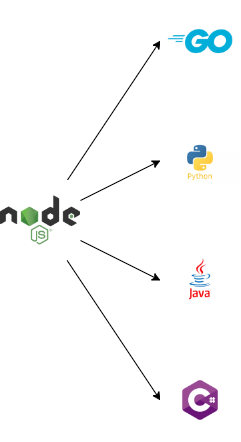
\includegraphics[height=3cm]{pictures/DaNgonNgu/_DaNgonNgu.png}
        \caption{ViDuHinhAnhTheoChieuDoc}  
        % % Thêm vào hình SQL riêng 
        \end{figure} 
        
       


        
        
        


    \end{itemize}
\end{itemize}

%     \item Các  
% 
%                         %     $VD: 




%                           \item Độc lập về     triển khai hệ thống



%                           Mỗi dịch vụ   triển khai độc lập và có thể thực hiện các thay đổi  mà không ảnh hưởng đến các dịch vụ khác.  





%           \end{itemize}
% \end{itemize}

% % Các dịch vụ ít phụ thuộc vào các dịch vụ khác.
% Giảm thiểu ràng buộc và tăng tính linh hoạt của hệ thống.
% Hệ thống có khả năng chịu lỗi cao tăng độ tin cậy.
% % Khả năng phục hồi : Kiến trúc phải được thiết kế để chịu đựng lỗi và các dịch vụ phải có khả năng xử lý lỗi một cách duyên dáng.
% Tính linh hoạt : Kiến trúc phải cho phép phát triển và triển khai nhanh chóng các dịch vụ mới cũng như khả năng thay đổi các dịch vụ hiện có một cách nhanh chóng và dễ dàng.
% \textbf{Từ đó    dễ dàng  mở rộng hệ thống.}
%%%%%%%%%%%%%%%%%%%%%%%%%%%%%%%%%%%%%



%%%%%%%%%%%%%%%%%%%%%%%%%%%%%%%%%%%%%


% Các dịch vụ tương tác với nhau qua hạ tầng mạng.

% Các dịch vụ tương tác với nhau qua hạ tầng mạng.

% Các dịch vụ tương tác với nhau qua hạ tầng mạng.

% Các dịch vụ tương tác với nhau qua hạ tầng mạng.

% Các dịch vụ tương tác với nhau qua hạ tầng mạng.

% Các dịch vụ tương tác với nhau qua hạ tầng mạng.

% Các dịch vụ tương tác với nhau qua hạ tầng mạng.

% Các dịch vụ tương tác với nhau qua hạ tầng mạng.

% Các dịch vụ tương tác với nhau qua hạ tầng mạng.

% \subsubsection{Một số nhược điểm và thách thức của kiến trúc vi dịch vụ}
% % Mặc dù kiến trúc vi dịch vụ có nhiều lợi ích nhưng  cũng có nhiều thách thức:

Chịu ảnh hưởng của đường truyền mạng.
Đồng bộ đồng hồ thời gian.
Ràng buộc về thứ tự sự kiện.
Tính nhất quán và toàn vẹn của dữ liệu.
Khả năng kiểm soát giao dịch.

Giám sát giữa các dịch vụ.
Bảo mật giao tiếp giữa các dịch vụ.


Phát hiện lỗi và sửa lỗi khó khăn, phức tạp hơn.




Chi phí xây dựng, quản lí vận hành lớn. 
 



% \subsubsection{Có thể thêm phần truyền thông trực tiếp, gián tiếp}

% \subsection{Giới thiệu về thiết kế hướng miền}
% Trong quá trình hoạt động kinh doanh, không phải mọi doanh nghiệp đều giữ nguyên mô hình kinh doanh được đưa ra ban đầu của mình. Khi quy mô thị trường thay đổi, việc chuyển đổi mô hình kinh doanh là điều cần thiết. Chuyển đổi kinh doanh như một công cụ linh hoạt giúp các doanh nghiệp có thể phát triển và tồn tại giữa các đối thủ của mình.

Ví dụ:






\begin{itemize}
    \item   Google bắt đầu như một công cụ tìm kiếm trực tuyến, nhưng sau đó đã mở rộng và thay đổi mô hình kinh doanh qua nhiều dịch vụ và sản phẩm khác nhau như: Dịch vụ đám mây Google Cloud Platform, thư điện tử Gmail, bản đồ Google Maps, lưu trữ tập tin Google Drive, \dots
    \item   Amazon từ hiệu sách trực tuyến đã trở thành thị trường cho nhà cung cấp khác như: Thương mại điện tử, Dịch vụ đám mây Amazon Web Services (AWS), \dots
\end{itemize}

\begin{figure}[h]

    \centering

    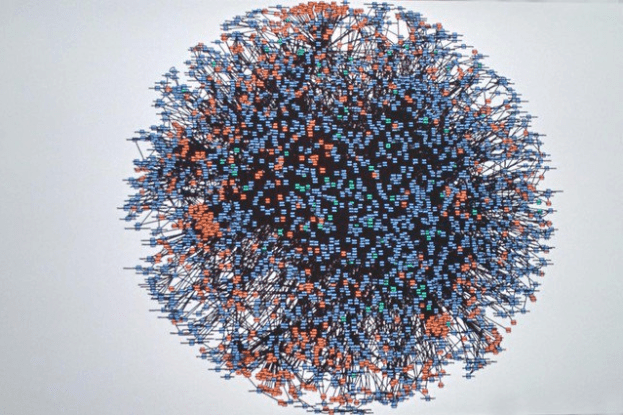
\includegraphics[width = 0.5\textwidth]{pictures/KienTrucViDichVuAmazon/main.png}

    \caption{Kiến trúc vi dịch vụ của Amazon}

\end{figure}


Đối với những doanh nghiệp không chuyển đổi kinh doanh sẽ không thể tồn tại.

Ví dụ: Gần đây, Baemin dịch vụ giao đồ ăn đã rời khỏi thị trường Việt Nam cũng do sức ép từ các đối thủ khác khiến Baemin khó cạnh tranh trong mảng kinh doanh cốt lõi là giao đồ ăn. Các đối thủ này không chỉ cung cấp dịch vụ giao đồ ăn mà còn có đặt xe, giao hàng,...


\begin{figure}[h]
    
    \centering
    
    % ![](pictures/Baemin.png)
    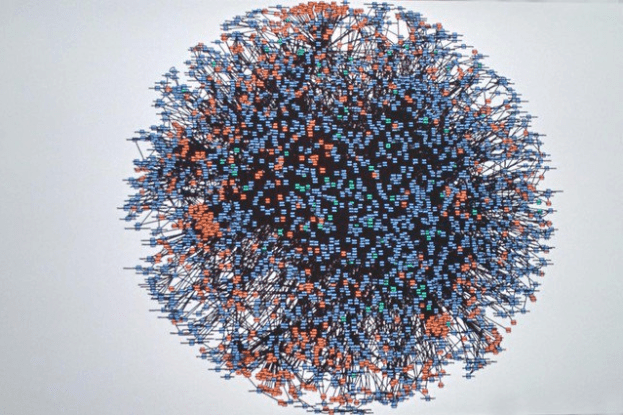
\includegraphics[width = 0.5\textwidth]{pictures/KienTrucViDichVuAmazon/main.png}

    \caption{  Baemin đã rời khỏi thị trường Việt Nam}

\end{figure}

%%%%%%%%%%%%%%%%%%%%%%%%%%%%%%%%%%%%%

% = > Hiện nay, các tổ chức doanh nghiệp có nhu cầu phát triển chuyển đổi kinh doanh để có thể tồn tại và phát triển khi thị trường thay đổi. Từ đó, đáp ứng nhu cầu của khách hàng, giúp mang đến ưu thế cạnh tranh so với các đối thủ. Do đó cần hệ thống chuyển đổi nhanh chóng đáp ứng nhu cầu của dự án và mong đợi của khách hàng.

% = > Kiến trúc vi dịch vụ giải quyết những thách thức và hỗ trợ doanh nghiệp chuyển đổi dễ dàng.

%%%%%%%%%%%%%%%%%%%%%%%%%%%%%%%%%%%%%

Tuy nhiên, để xây dựng được kiến trúc vi dịch vụ tốt cần phải tạo ra các dịch vụ nhỏ phù hợp và duy trì tính độc lập. Nếu không thực hiện đúng các nhóm phụ thuộc lẫn nhau và mất đi lợi thế của kiến trúc vi dịch vụ.

Và từ đó, mẫu thiết kế hướng miền sử dụng để phân tích xây dựng kiến trúc vi dịch vụ.

Thiết kế hướng miền xác định và tổ chức các dịch vụ dựa trên việc hiểu rõ về lĩnh vực kinh doanh, giúp dự án phản ánh đúng các quy trình và quy tắc kinh doanh.

%%%%%%%%%%%%%%%%%%%%%%%%%%%%%%%%%%%%%

% thiết kế hướng miền có thể trợ giúp như thế nào

% Thiết kế hướng miền (thiết kế hướng miền) có thể hỗ trợ kiến trúc và thiết kế kiến trúc vi dịch vụ theo nhiều cách:

% Bối cảnh giới hạn : thiết kế hướng miền nhấn mạnh việc xác định các bối cảnh giới hạn, là các khu vực riêng biệt của miền có ranh giới được xác định rõ ràng. Điều này có thể giúp xác định ranh giới của kiến trúc vi dịch vụ và đảm bảo rằng mỗi kiến trúc vi dịch vụ đều có trách nhiệm rõ ràng và tập trung.

% ngôn ngữ chung : thiết kế hướng miền khuyến khích sử dụng một ngôn ngữ chung được chia sẻ bởi cả chuyên gia ngành và nhân viên kỹ thuật. Điều này có thể giúp đảm bảo rằng các vi dịch vụ giao tiếp hiệu quả với nhau và phù hợp với yêu cầu kinh doanh.

% Ánh xạ bối cảnh: thiết kế hướng miền cung cấp các kỹ thuật để ánh xạ các mối quan hệ giữa các bối cảnh giới hạn. Điều này có thể giúp đảm bảo rằng các vi dịch vụ được thiết kế với sự hiểu biết rõ ràng về sự phụ thuộc của chúng vào các dịch vụ khác.

% Tập hợp: thiết kế hướng miền định nghĩa tập hợp là các cụm đối tượng liên quan cần được coi là một đơn vị nhất quán duy nhất. Điều này có thể giúp đảm bảo rằng các vi dịch vụ được thiết kế với sự hiểu biết rõ ràng về các yêu cầu về tính nhất quán của dữ liệu.

% Tương quan với bối cảnh giới hạn

% Mặc dù người ta thường khuyên nên căn chỉnh ranh giới của kiến trúc vi dịch vụ với ranh giới của bối cảnh giới hạn, nhưng điều đó không phải lúc nào cũng cần thiết hoặc khả thi. Một vi dịch vụ có thể gói gọn nhiều ngữ cảnh giới hạn hoặc một ngữ cảnh giới hạn có thể được phân chia thành nhiều vi dịch vụ, tùy thuộc vào nhu cầu cụ thể của hệ thống và sự cân bằng liên quan. Cuối cùng, mục tiêu là tạo ra một hệ thống mô - đun và có thể bảo trì, đáp ứng các yêu cầu kinh doanh và mối quan hệ giữa bối cảnh giới hạn và các vi dịch vụ phải được thiết kế phù hợp.

% Tương quan với API thực thể

% Nhìn chung, việc thiết kế các vi dịch vụ chỉ dựa trên các hoạt động CRUD của thực thể không được khuyến khích vì nó có thể dẫn đến một kiến trúc liên kết chặt chẽ và không hiệu quả. Các vi dịch vụ phải được thiết kế dựa trên khả năng kinh doanh, có thể phù hợp hoặc không phù hợp với hoạt động CRUD của thực thể.

% thiết kế hướng miền có thể giúp xác định các khả năng kinh doanh và xác định bối cảnh giới hạn, sau đó có thể được sử dụng để hướng dẫn thiết kế các vi dịch vụ. Bằng cách tập trung vào khả năng kinh doanh thay vì hoạt động CRUD thực thể, các vi dịch vụ có thể được liên kết lỏng lẻo hơn, mang tính mô - đun hơn, dễ dàng duy trì và phát triển hơn theo thời gian.



%%%%%%%%%%%
% \section{Yêu cầu nghiệp vụ}
% Yêu cầu nghiệp vụ xác định nội dung, phạm vi, mục tiêu và chức năng mong muốn của hệ thống.

% Nguồn: TCT

% \subsection {Yêu cầu nghiệp vụ của bài toán phụ}
% Trang web "https: //hoadondientu.gdt.gov.vn" là trang web do Tổng Cục Thuế quản lý và sử dụng để thực hiện các quy trình liên quan đến thuế điện tử. Thực tế, yêu cầu đăng ký chính thức từ Tổng Cục Thuế dành cho cá nhân và doanh nghiệp. Vì em không có tài khoản chính thức nên ở đồ án này, em sẽ tạo  tong-cuc-thue-demo - một phiên bản giả lập của hệ thống chính thức, dành cho mục đích học tập phục vụ cho bài toán chính là "Xây dựng kiến trúc vi dịch vụ cho bài toán hóa đơn điện tử".


% \subsubsection{Các chức năng tổng quan của bài toán phụ}
% Để đơn giản hóa bài toán, các chức năng trong đồ án này đã thay đổi so với bài toán thực tế trong tài liệu hướng dẫn sử dụng cổng thông tin điện tử của TCT cho hóa đơn điện tử:

\textbf{Em đã bỏ qua hình thức hóa đơn}

Hóa đơn có mã của cơ quan thuế

Hóa đơn không có mã của cơ quan thuế

\textbf{Bỏ qua các loại hóa đơn khác nhau}

Hóa đơn điện tử giá trị gia tăng

Hóa đơn bán hàng

Hóa đơn bán tài sản công

Hóa đơn bán hàng dự trữ quốc gia

Hóa đơn khác

Phiếu xuất kho kiêm vận chuyển nội bộ

Phiếu xuất kho gửi bán hàng đại lý

\textbf{Bỏ qua phần ký số}

USB Token hay còn gọi là chữ ký số Token là một thiết bị mà mọi doanh nghiệp, tổ chức hiện nay đều cần phải có để thực hiện khai báo và nộp thuế điện tử, cũng như để giao dịch với khách hàng.

\textbf{Bỏ qua phần ký hiệu hóa đơn}

Vì mục đích của ký hiệu hóa đơn là nhóm 6 ký tự thể hiện thông tin về loại hóa đơn điện tử có mã hoặc không mã, năm lập hóa đơn, loại hóa đơn.

\textbf{Bỏ qua chức năng lập hóa đơn điều chỉnh}

E bỏ qua chức năng lập hóa đơn điều chỉnh và chỉ có chức năng lập hóa đơn thay thế.

\textbf{Bỏ qua chức năng phê duyệt hóa đơn}

\textbf{Bỏ qua định dạng file XML,PDF,HTML, EXCEL}

\textbf{Tóm lại, các chức năng tổng quan của tong - cuc - thue - demo bao gồm:}

\underline{\textsc{QUẢN LÝ TÀI KHOẢN}}

Đăng ký

% mail active

% active

Đăng nhập

Đăng xuất

Quên mật khẩu

% mail reset

% reset

Đổi mật khẩu

Thay đổi thông tin

\underline{\textsc{QUẢN LÝ HỆ THỐNG}}

Quản lý vai trò

Quản lý người dùng

\underline{\textsc{QUẢN LÝ DANH MỤC}}

Danh mục khách hàng

Danh mục hàng hóa

\underline{\textsc{QUẢN LÝ HÓA ĐƠN}}

Lập hóa đơn mới

Lập hóa đơn thay thế

Hủy hóa đơn

\underline{\textsc{TRA CỨU HÓA ĐƠN}}

Tra cứu hóa đơn khi NNT chưa đăng nhập

Tra cứu hóa đơn khi NNT đã đăng nhập

\underline{\textsc{GỬI PHẢN HỒI QUA THƯ ĐIỆN TỬ}}

Gửi thông tin của TCT đến NNT
% \subsection{Yêu cầu nghiệp vụ chưa xong}
% \subsection{Yêu cầu nghiệp vụ chưa xong}
% \subsection{Yêu cầu nghiệp vụ chưa xong}
% \subsection{Yêu cầu nghiệp vụ chưa xong}
% \subsection{Yêu cầu nghiệp vụ chưa xong}
% chưa xong
% %@ %@ %@ %@ %@ %@ Mẫu mail

%!<! - - // NNT nhận được thư điện tử của CQT thông báo tiếp nhận tờ khai đăng ký - - >

Trong thời gian 15 phút kể từ khi nhận được tờ khai đăng ký của NNT, Cổng điện tử gửi thư điện tử thông báo về việc tiếp nhận/không tiếp nhận tờ khai đăng ký của NNT.

Nội dung mẫu:

```
Tiêu đề: (TCT Demo) Thông báo về việc tiếp nhận tờ khai đăng ký sử dụng hóa đơn điện tử
Kính gửi: {{Tên NNT}}
Mã số thuế: {{Mã số thuế}}

Căn cứ Tờ khai đăng ký sử dụng hóa đơn điện tử - Ban hành kèm theo Nghị định số 123/2020/NĐ - CP của người nộp thuế (NNT) gửi tới cơ quan thuế ngày {{Ngày nhận}}, cơ quan thuế tiếp nhận Tờ khai đăng ký sử dụng hóa đơn điện tử của NNT, cụ thể như sau:
Tên tờ khai: Tờ khai đăng ký sử dụng hóa đơn điện tử
Mã giao dịch điện tử: {{Mã số thuế + Thời gian}}

Cơ quan thuế thông báo để NNT được biết và thực hiện.
```

%!<! - - NNT nhận được thư điện tử của CQT chấp nhận/không chấp nhận đăng ký sử dụng HĐĐT - - >

Trong thời gian 01 ngày làm việc kể từ ngày Cổng điện tử gửi thông báo về việc tiếp nhận, cơ quan thuế quản lý sẽ gửi thông báo về việc chấp nhận/không chấp nhận đăng ký sử dụng hóa đơn điện tử.

Nội dung mẫu chấp nhận đăng ký sử dụng HĐĐT:

```
Tiêu đề: (TCT Demo) Thông báo về việc chấp nhận đăng ký sử dụng hóa đơn điện tử
Kính gửi: {{Tên NNT}}
Mã số thuế: {{Mã số thuế}}

Sau khi xem xét tờ khai đăng ký sử dụng hóa đơn điện tử của NNT gửi đến cơ quan thuế ngày {{Ngày nhận}}.
Cơ quan thuế thông báo chấp nhận đề nghị đăng ký sử dụng hóa đơn điện tử của NNT.

Cơ quan thuế thông báo để NNT được biết và thực hiện.
```

Nội dung mẫu không chấp nhận đăng ký sử dụng HĐĐT:

```
Tiêu đề: (TCT Demo) Thông báo về việc không chấp nhận đăng ký sử dụng hóa đơn điện tử
Kính gửi: {{Tên NNT}}
Mã số thuế: {{Mã số thuế}}

Sau khi xem xét tờ khai đăng ký sử dụng hóa đơn điện tử của NNT gửi đến cơ quan thuế ngày {{Ngày nhận}}.
Cơ quan thuế thông báo không chấp nhận đề nghị đăng ký sử dụng hóa đơn điện tử của NNT.

Cơ quan thuế thông báo để NNT được biết và thực hiện.
```

%!<! - - NNT nhận được Thông báo tài khoản sử dụng tra cứu HĐĐT trên cổng thông tin điện tử của TCT - - >

Sau khi NNT nhận được thông báo về việc chấp nhận đăng ký sử dụng hóa đơn điện tử, cơ quan thuế gửi thông báo tài khoản sử dụng của NNT qua thư điện tử bao gồm Tên tài khoản và Mật khẩu.

Nội dung mẫu:

```
Tiêu đề: (TCT Demo) Thông báo tài khoản sử dụng tra cứu HĐĐT trên cổng thông tin điện tử của TCT
Kính gửi: {{Tên NNT}}
Mã số thuế: {{Mã số thuế}}

Sau khi xem xét tờ khai đăng ký sử dụng hóa đơn điện tử cơ quan thuế tiếp nhận ngày {{Ngày nhận}}.
Cơ quan thuế thông báo chấp nhận đề nghị đăng ký sử dụng hóa đơn điện tử của NNT và gửi thông tin tài khoản sử dụng tra cứu HĐĐT trên cổng thông tin điện tử của TCT như sau:
Tên tài khoản: {{admin + Mã số thuế}}
Mật khẩu: {{Mật khẩu}}

Cơ quan thuế thông báo để NNT được biết và thực hiện.
```

%!<! - - - - >
%!<! - - - - >
%!<! - - - - >
%!<! - - - - >
%!<! - - - - >
%!<! - - - - >
%!<! - - - - >
%!<! - - - - >
%!<! - - - - >
%!<! - - - - >

%!<! - - NNT nhận được thư điện tử của CQT thông báo tiếp nhận tờ khai đăng ký thay đổi - - >

Trong thời gian 15 phút kể từ khi nhận được tờ khai đăng ký của NNT, Cổng điện tử gửi thư điện tử thông báo về việc tiếp nhận/không tiếp nhận tờ khai đăng ký thay đổi thông tin đăng ký sử dụng của NNT.

Nội dung mẫu:

```
Tiêu đề: (TCT Demo) Thông báo về việc tiếp nhận tờ khai đăng ký thay đổi thông tin đăng ký sử dụng của NNT
Kính gửi: {{Tên NNT}}
Mã số thuế: {{Mã số thuế}}

Căn cứ Tờ khai đăng ký thay đổi thông tin đăng ký sử dụng của NNT gửi tới cơ quan thuế ngày {{Ngày nhận}}, cơ quan thuế tiếp nhận Tờ khai đăng ký sử dụng hóa đơn điện tử của NNT, cụ thể như sau:
Tên tờ khai: Tờ khai đăng ký thay đổi thông tin đăng ký sử dụng của NNT
Mã giao dịch điện tử: {{Mã số thuế + Thời gian}}

Cơ quan thuế thông báo để NNT được biết và thực hiện.
```

%!<! - - NNT nhận được thư điện tử của CQT chấp nhận/không chấp nhận đăng ký sử dụng HĐĐT - - >

Trong thời gian 01 ngày làm việc kể từ ngày Cổng điện tử gửi thông báo về việc tiếp nhận, cơ quan thuế quản lý sẽ gửi thông báo về việc chấp nhận/không chấp nhận đăng ký thay đổi thông tin đăng ký sử dụng của NNT.

Nội dung mẫu chấp nhận đăng ký thay đổi thông tin đăng ký sử dụng của NNT

```
Tiêu đề: (TCT Demo) Thông báo về việc chấp nhận đăng ký thay đổi thông tin đăng ký sử dụng của NNT
Kính gửi: {{Tên NNT}}
Mã số thuế: {{Mã số thuế}}

Sau khi xem xét tờ khai đăng ký thay đổi thông tin đăng ký sử dụng của NNT gửi đến cơ quan thuế ngày {{Ngày nhận}}.
Cơ quan thuế thông báo chấp nhận đề nghị đăng ký thay đổi thông tin đăng ký sử dụng của NNT.

Cơ quan thuế thông báo để NNT được biết và thực hiện.
```

Nội dung mẫu không chấp nhận đăng ký thay đổi thông tin đăng ký sử dụng của NNT

```
Tiêu đề: (TCT Demo) Thông báo về việc không chấp nhận đăng ký thay đổi thông tin đăng ký sử dụng của NNT
Kính gửi: {{Tên NNT}}
Mã số thuế: {{Mã số thuế}}

Sau khi xem xét tờ khai đăng ký thay đổi thông tin đăng ký sử dụng của NNT gửi đến cơ quan thuế ngày {{Ngày nhận}}.
Cơ quan thuế thông báo không chấp nhận đề nghị đăng ký thay đổi thông tin đăng ký sử dụng của NNT.

Cơ quan thuế thông báo để NNT được biết và thực hiện.
```

%!<! - - - - >
%!<! - - - - >
%!<! - - - - >
%!<! - - - - >
%!<! - - - - >
%!<! - - - - >
%!<! - - - - >

%!<! - - Sau khi gửi yêu cầu lấy lại mật khẩu NNT sẽ nhận được thông báo của CQT qua gửi thư điện tử - - >

Nội dung mẫu:

```
Tiêu đề: (TCT Demo) Thông báo về việc lấy lại mật khẩu
Kính gửi: {{Tên NNT}}
Mã số thuế: {{Mã số thuế}}

Sau khi xem xét yêu cầu lấy lại mật khẩu của NNT gửi đến cơ quan thuế ngày {{Ngày nhận}}.
Cơ quan thuế gửi thông tin tài khoản sử dụng tra cứu HĐĐT trên cổng thông tin điện tử của TCT như sau:
Tên tài khoản: {{Tên tài khoản}}
Mật khẩu mới: {{Mật khẩu mới}}

Cơ quan thuế thông báo để NNT được biết và thực hiện.
```

%@ %@ %@ Chi tiết các chức năng của TCT Demo:

Chi tiết các chức năng của TCT Demo:

QUẢN LÝ TÀI KHOẢN

Quản lý tài khoản là một chức năng phổ biến trong nhiều ứng dụng. Chức năng này đảm bảo tính bảo mật và an toàn trong việc sử dụng tài khoản.

%!<! - - Chức năng: "Đăng ký sử dụng hóa đơn điện tử" - - >

NNT nhập MST có 10 ký tự cho cá nhân, doanh nghiệp hoặc 14 ký tự cho chi nhánh của doanh nghiệp với định dạng "Mã số thuế doanh nghiệp - Mã chi nhánh".
Ví dụ:
Mã số thuế 10 ký tự: 0123456789
Mã số thuế 14 ký tự: 0123456789 - 001

Hệ thống tự động hiển thị thông tin Đăng ký thuế của NNT bao gồm "Tên của NNT", "Mã cơ quan thuế quản lý" và "Tên cơ quan thuế quản lý".

Tiếp theo, NNT nhập các thông tin hợp lệ: "Người liên hệ", "Điện thoại liên hệ", "Địa chỉ liên hệ", "Thư điện tử".

Cuối cùng, NNT gửi đăng ký với thông tin "Ngày thực hiện" là ngày NNT đang đăng ký hóa đơn điện tử.

Sau khi gửi thông tin đăng kí NNT sẽ nhận được thông báo làm việc của CQT qua gửi thư điện tử về việc tiếp nhận và chấp nhận đăng ký, cùng với tài khoản và mật khẩu cho NNT.

%!<! - - // Nếu mã số thuế không đúng định dạng, hệ thống sẽ thông báo: "Mã số thuế phải có độ dài 10 hoặc 14 ký tự và đúng định dạng". - - >
%!<! - - // Nếu mã số thuế tồn tại, hệ thống kiểm tra xem NNT đã đăng ký sử dụng hóa đơn điện tử khác chưa. Nếu đã tồn tại tờ khai đăng ký, hệ thống thông báo: "Đã tồn tại tờ khai đăng ký sử dụng hóa đơn điện tử khác của NNT đã được cơ quan thuế chấp nhận". - - >

%!<! - - // Người liên hệ: phải chứa một chuỗi kí tự và không được để trống. - - >
%!<! - - // Điện thoại liên hệ: phải chứa một chuỗi kí tự số và dấu " + " ở đầu chuỗi (nếu có) và không được để trống. - - >
%!<! - - // Địa chỉ liên hệ: phải chứa một chuỗi kí tự và không được để trống. - - >
%!<! - - // Thư điện tử: phải chứa một chuỗi kí tự có định dạng email và không được để trống. - - >

%!<! - - // Khi NNT nhấn nút "Ký gửi", hệ thống sẽ hiển thị thông báo hỏi "Xác nhận ký gửi" với hai lựa chọn là "Đồng ý" hoặc "Hủy bỏ". - - >
%!<! - - // Nếu NNT chọn "Đồng ý", hệ thống sẽ thông báo: "Gửi thông tin đăng ký sử dụng hóa đơn điện tử cho cơ quan thuế thành công". - - >

%!<! - - - - >
%!<! - - Chức năng: "Thay đổi đăng ký sử dụng hóa đơn điện tử" - - >

Trong quá trình sử dụng hóa đơn điện tử, khi NNT muốn thay đổi đăng ký sử dụng hóa đơn, họ có thể sử dụng chức năng "Thay đổi đăng ký sử dụng hóa đơn điện tử".

NNT Nhập thông tin có thể thay đổi, bao gồm: Tên NNT, Người liên hệ, Điện thoại liên hệ, Địa chỉ liên hệ, Thư điện tử.
Cuối cùng, NNT gửi đăng ký thay đổi với thông tin "Ngày thực hiện" là ngày NNT đang đăng ký thay đổi hóa đơn điện tử.

Sau khi gửi thông tin thay đổi đăng ký, NNT sẽ nhận được thông báo làm việc từ cơ quan thuế qua thư điện tử về việc tiếp nhận và chấp nhận thay đổi đăng ký cho NNT.

%!<! - - Chức năng: "Đăng nhập tài khoản" - - >

Sau khi CQT gửi thư điện tử chứa tài khoản và mật khẩu cho NNT, NNT thực hiện nhập đầy đủ thông tin bao gồm: Tên đăng nhập, Mật khẩu để thực hiện việc đăng nhập vào tài khoản.

%!<! - - Chức năng: "Đăng xuất tài khoản" - - >

Chức năng để NNT đăng xuất tài khoản.

%!<! - - Chức năng: "Đổi mật khẩu" - - >

NNT cung cấp đầy đủ thông tin bao gồm: Mật khẩu cũ, Mật khẩu mới và Nhập lại mật khẩu mới để thực hiện việc thay đổi mật khẩu.

%!<! - - Chức năng: "Quên mật khẩu" - - >

NNT cung cấp đầy đủ thông tin bao gồm: Tên đăng nhập, Thư điện tử. Sau đó, nhấn "Quên mật khẩu" để khôi phục mật khẩu. CQT gửi mật khẩu mới về email của NNT.

%!<! - - QUẢN LÝ HỆ THỐNG - - >

%!<! - - Chức năng: "Quản lý vai trò" - - >

Người quản trị hệ thống (admin) là một vai trò cố định được phép sử dụng tất cả các chức năng trên Cổng điện tử.
Người quản trị hệ thống có thể thực hiện CRUD "Vai trò" với các thông tin bao gồm: "ID", "Tên vai trò" và "Quyền".

Các quyền bao gồm:
Thay đổi đăng ký sử dụng hóa đơn điện tử
Quản lý vai trò
Quản lý người dùng
Quản lí danh mục
Quản lí hóa đơn
Tra cứu hóa đơn

%!<! - - Chức năng: "Quản lý người dùng" - - >

Người quản trị hệ thống có thể thực hiện CRUD "Người dùng" với các thông tin bao gồm: "Tên người dùng", "Mật khẩu", "Điện thoại", "Thư điện tử" và "Vai trò".

%!<! - - QUẢN LÝ DANH MỤC - - >

%!<! - - Chức năng: "Danh mục khách hàng" - - >

Chức năng này thực hiện CRUD "Khách hàng" có các thông tin: "Mã khách hàng", "Tên khách hàng", "Mã số thuế", "Tên NNT", "Địa chỉ", "SĐT khách hàng", Số tài khoản, Ngân hàng

%!<! - - Chức năng: "Danh mục hàng hóa" - - >

Chức năng này thực hiện CRUD "Hàng hóa" có các thông tin: "Mã hàng hóa, dịch vụ", "Tên hàng hóa, dịch vụ", "Đơn vị tính", "Đơn giá", "Thuế suất".

%!<! - - QUẢN LÝ HÓA ĐƠN ĐIỆN TỬ - - >

%!<! - - Chức năng: "Lập hóa đơn mới" - - >

Nhập thông tin người bán: MST người bán, Tên người bán, Địa chỉ người bán, Số điện thoại người bán.

Nhập thông tin người mua: Mã khách hàng, Tên khách hàng, Mã số thuế, Địa chỉ khách hàng, SĐT khách hàng.

Nhập thông tin hàng hóa, dịch vụ: "Số thứ tự", "Mã hàng hóa, dịch vụ", "Tên hàng hóa, dịch vụ", "Đơn vị tính", "Đơn giá", "Thuế suất" và "Số lượng".

Hệ thống tự động tính toán:

- Ngày lập hóa đơn sẽ tự động là ngày hiện tại khi người lập tạo hóa đơn mới.

- Tổng tiền trước thuế.

- Tổng tiền sau thuế.

%!<! - - Chức năng: "Lập hóa đơn thay thế" - - >

Chức năng này cho phép thay đổi các thông tin trong hóa đơn gốc.

Lưu ý:

- Hãy lưu trữ thông tin ID của hóa đơn thay thế trong trạng thái "Bị thay thế" của hóa đơn gốc.

- Hãy lưu trữ thông tin ID của hóa đơn gốc trong trạng thái "Thay thế" của hóa đơn thay thế.

%!<! - - Chức năng: "Hủy hóa đơn" - - >

Chức năng này cho phép xóa hóa đơn và các hóa đơn thay thế liên quan.

%!<! - - TRA CỨU HÓA ĐƠN - - >

Người sử dụng có thể thực hiện tra cứu hóa đơn trên cổng thông tin điện tử theo 2 cách:
Cách 1: Tra cứu hóa đơn khi NNT chưa đăng nhập
Cách 2: Tra cứu hóa đơn khi NNT đã đăng nhập

%!<! - - Chức năng: "Tra cứu hóa đơn khi NNT chưa đăng nhập" - - >

%!<! - - Tra cứu thông tin hóa đơn - - >

Người tra cứu nhập thông tin bao gồm: Mã số thuế người bán, Số hóa đơn, Tổng tiền thuế, Tổng tiền thanh toán, Ngày lập hóa đơn.

%!<! - - Kết quả: - - >
%!<! - - - Nếu hóa đơn điện tử không hợp lệ, hệ thống sẽ hiển thị thông báo: "Không tồn tại hóa đơn có thông tin trùng khớp với các thông tin tổ chức, cá nhân tìm kiếm”. - - >
%!<! - - - Nếu hóa đơn điện tử hợp lệ, hệ thống sẽ hiển thị thông báo: "Tồn tại hóa đơn có thông tin trùng khớp với các thông tin tổ chức, cá nhân tìm kiếm". - - >
%!<! - - - Nếu hóa đơn tìm kiếm là hóa đơn thay thế, bị thay thế hệ thống sẽ hiển thị thông tin bổ sung về hóa đơn liên quan: "Hóa đơn này là hóa đơn thay thế cho hóa đơn có ID: {{ID}}" hoặc "Hóa đơn này là hóa đơn bị thay thế của hóa đơn có ID: {{ID}}". - - >

%!<! - - Tra cứu thông tin "Mã số thuế" - - >

Người tra cứu nhập thông tin bao gồm: Mã số thuế.

%!<! - - Kết quả: - - >
%!<! - - - Nếu đã đăng kí, hệ thống sẽ hiển thị thông báo: “MST 0107001729 đã đăng ký sử dụng hóa đơn điện tử theo Nghị định 123/2020/NĐ - CP". - - >
%!<! - - - Nếu NNT chưa đăng kí hoặc đã đăng kí nhưng cơ quan thuế có thông báo về việc không được chấp nhận đăng kí sử dụng hóa đơn điện tử, hệ thống sẽ hiển thị thông báo: “MST 0107001728 chưa sử dụng hóa đơn điện tử theo Nghị định 123/2020/NĐ - CP". - - >
%!<! - - Chức năng: "Tra cứu hóa đơn khi NNT đã đăng nhập" - - >

Cổng điện tử hỗ trợ tra cứu 2 loại hóa đơn là hóa đơn bán ra và hóa đơn mua vào.

Người tra cứu nhập thông tin tra cứu bao gồm: Mã số thuế người bán, Ngày lập hóa đơn và Số hóa đơn.

Cổng điện tử hỗ trợ các chức năng sau: Xem thông tin hóa đơn, In hóa đơn và Xuất hóa đơn (định dạng Excel, XML, PDF).

%!<! - - GỬI PHẢN HỒI QUA THƯ ĐIỆN TỬ - - >

%!<! - - - Gửi thông tin làm việc của TCT cho yêu cầu của NNT - - >

%!<! - - $ NNT nhận được thư điện tử của CQT thông báo tiếp nhận tờ khai đăng ký - - >

%!<! - - $ NNT nhận được thư điện tử của CQT chấp nhận/không chấp nhận đăng ký sử dụng HĐĐT - - >

%!<! - - $ NNT nhận được Thông báo tài khoản sử dụng tra cứu HĐĐT trên cổng thông tin điện tử của TCT - - >

%!<! - - $ NNT nhận được thư điện tử của CQT thông báo tiếp nhận tờ khai đăng ký thay đổi - - >

%!<! - - $ NNT nhận được thư điện tử của CQT chấp nhận/không chấp nhận đăng ký sử dụng HĐĐT - - >
%!<! - - Yêu cầu nghiệp vụ của bài toán chính - - >

%!<! - - Các chức năng của bài toán chính - - >

%!<! - - THÔNG BÁO - - >

Chức năng CRUD "Thông báo" bao gồm các thông tin: ID, tiêu đề, nội dung, thời gian.

%!<! - - QUẢN LÝ TÀI KHOẢN - - >

Tương tự " TCT Demo" với các chức năng sau:

Đăng ký
Đăng nhập
Đăng xuất
Quên mật khẩu
Xem thông tin
Thay đổi thông tin
Đổi mật khẩu

%!<! - - CẤU HÌNH EMAIL - - >

Cấu hình bao gồm:

Địa chỉ email
Mật khẩu email

Loại email gửi:

Xác nhận tài khoản mới
Quên mật khẩu
Gửi thông tin hóa đơn cho khách hàng

%!<! - - QUẢN LÝ DANH MỤC - - >

Tương tự " TCT Demo" bao gồm:

Danh mục khách hàng
Danh mục hàng hóa

%!<! - - QUẢN LÝ HỆ THỐNG - - >

Tương tự " TCT Demo" nhưng có thêm quyền "Cấu hình Email".

%!<! - - QUẢN LÝ HÓA ĐƠN ĐIỆN TỬ - - >

Tương tự " TCT Demo"

%!<! - - TRA CỨU HÓA ĐƠN - - >

Có 3 cách tra cứu:

Tra cứu 1 hóa đơn theo "Mã hóa đơn"
Tra cứu tất cả hóa đơn bán ra
Tra cứu tất cả hóa đơn mua vào

%!<! - - BÁO CÁO VÀ PHÂN TÍCH HÓA ĐƠN - - >

Các chức năng bao gồm:

Số lượng hóa đơn đã sử dụng
Tổng tiền trước thuế
Tổng tiền sau thuế
Tổng số tiền thuế
Số lượng khách hàng
Số lượng sản phẩm

%@ %@ %@ Tự động

Nghiệp vụ của bài toán chính
Các chức năng của bài toán chính
THÔNG BÁO
CRUD thông báo có (id, tiêu đề, nội dung, thời gian)
TÀI KHOẢN
Sử dụng tài khoản của " TCT Demo" với các chức năng tương tự Đăng ký, Đăng nhập, Đăng xuất, Quên mật khẩu, Xem thông tin, Thay đổi thông tin, Đổi mật khẩu
CẤU HÌNH EMAIL ĐỂ GỬI HÓA ĐƠN CHO KHÁCH HÀNG

Địa chỉ email
Mật khẩu email
CHỨC NĂNG DANH MỤC
Giống với " TCT Demo" gồm "Danh mục khách hàng" và "Danh mục hàng hóa"
TRA CỨU HÓA ĐƠN:
Có 3 cách tra cứu:
Tra cứu 1 hóa đơn theo "Mã hóa đơn".
Tra cứu tất cả hóa đơn bán ra.
Tra cứu tất cả hóa đơn mua vào.
BÁO CÁO VÀ PHÂN TÍCH HÓA ĐƠN

Số lượng hóa đơn đã sử dụng
Tổng trước thuế
Tổng sau thuế
Tổng số tiền thuế
Số lượng khách hàng
Số lượng sản phẩm

%!<! - - - - >
%!<! - - Phân quyền - - >
%!<! - - Thay đổi - - >
%!<! - - Lập hóa đơn mới - - >
%!<! - - Tra cứu - - >
%!<! - - mail - - >

%@ %@ %@ 4. Các sơ đồ phân tích thiết kế hệ thống

%@ %@ %@ %@ %@ %@ 4.1. UML Use Case Diagrams

%@ %@ %@ %@ %@ %@ 4.2. UML Activity Diagrams

%@ %@ %@ %@ %@ %@ 4.3. UML Sequence Diagrams

%@ %@ %@ %@ %@ %@ 4.4. UML Class Diagrams


%%%%%%%%%%%
% \section{Chi tiết và áp dụng thiết kế hướng miền}
% https:// thiết kế hướng miền - practitioners.com/home/glossary
% https: //www.infoq.com/minibooks/domain - driven - design - quickly

% \subsection{Đôi nét về thiết kế hướng miền (DomainDrivenDesign)}
% % Thiết kế hướng miền được Eric Evans giới thiệu trong cuốn sách "DomainDrivenDesign: Tackling Complexity in the Heart of Software".

Thiết kế hướng miền (DomainDrivenDesign) là một phương pháp thiết kế phần mềm tập trung vào việc hiểu rõ và mô hình hóa lĩnh vực kinh doanh của một tổ chức.

Thiết kế hướng miền nhấn mạnh việc sử dụng lĩnh vực nghiệp vụ kinh doanh để thảo luận và đề xuất giải pháp đáp ứng nhu cầu. Vì để tạo một phần mềm tốt, chúng ta cần phải hiểu rõ về chính phần mềm đó. Chính vì vậy để đạt được kết quả như mong đợi, chúng ta thường bắt đầu từ yêu cầu nghiệp vụ.

Trong nhiều ứng dụng thường có phần xử lý các công việc không liên quan đến vấn đề nghiệp vụ như truy cập file, hạ tầng mạng, CSDL,... trong đối tượng nghiệp vụ kinh doanh. Cách này giúp tốc độ hoàn thiện ứng dụng nhanh. Tuy nhiên, cách này làm cho thiết kế bị mất đi tính hướng đối tượng trong thực tế với mức độ doanh nghiệp lớn. Đây là lý do thiết kế hướng miền trở nên quan trọng.

Trong kiến trúc vi dịch vụ, thiết kế hướng miền giúp đảm bảo rằng mỗi dịch vụ được thiết kế phản ánh một phần cụ thể của lĩnh vực kinh doanh. Mỗi dịch vụ được quản lí bởi một nhóm nhỏ được hỗ trợ bởi các chuyên gia ngành.

% %!<! - - Domain - Driven Design : https:// thiết kế hướng miền - practitioners.com/domain - driven - design - - >

% thường được sử dụng trong các dự án phần mềm phức tạp, quy mô lớn trong đó lĩnh vực kinh doanh có tính đặc thù cao và phần mềm phải phản ánh chính xác các quy trình kinh doanh cơ bản.



% \subsection{Miền (Domain)}
% Phần mềm được tạo ra để xử lý sự phức tạp trong cuộc sống hiện đại. Việc phát triển phần mềm liên kết chặt chẽ với một số khía cạnh cụ thể trong cuộc sống của chúng ta.

Miền (Domain) đề cập đến phạm vi kiến thức và vấn đề mà hệ thống hoặc dự án cụ thể đang xử lý.

Về góc độ kinh doanh: miền đại diện cho một lĩnh vực hoặc ngành mà doanh nghiệp hoạt động.
Về góc độ phần mềm: miền có thể coi là đại diện cho không gian vấn đề của phần mềm đó.

Phần mềm cần phản ánh đúng miền và hiện thực hóa chính xác miền.

%!<! - - $VD: Ở đồ án này, miền được xác định là bài toán giải pháp hóa đơn điện tử. - - >

% %!<! - - Domain : https:// thiết kế hướng miền - practitioners.com/domain - - >
% %!<! - - Domain : https:// thiết kế hướng miền - practitioners.com/domain - - >
% %!<! - - Domain : https:// thiết kế hướng miền - practitioners.com/domain - - >
% %!<! - - Domain : https:// thiết kế hướng miền - practitioners.com/domain - - >
% %!<! - - Domain : https:// thiết kế hướng miền - practitioners.com/domain - - >
% %!<! - - Domain : https:// thiết kế hướng miền - practitioners.com/domain - - >
% %!<! - - Domain : https:// thiết kế hướng miền - practitioners.com/domain - - >
% %!<! - - Domain : https:// thiết kế hướng miền - practitioners.com/domain - - >

%!<! - - [[Domain]] A sphere of knowledge, influence, or activity. - - >

Trang chủTrang chủBảng chú giảiLãnh địa
Lãnh địa
Trong thiết kế hướng miền (thiết kế hướng miền), miền là một phạm vi kiến thức, ảnh hưởng hoặc hoạt động đại diện cho một lĩnh vực chuyên môn hoặc mối quan tâm cụ thể. Miền là không gian vấn đề mà phần mềm đang được xây dựng để giải quyết và nó thể hiện vấn đề hoặc cơ hội kinh doanh mà phần mềm có nhiệm vụ giải quyết.

Miền có thể là một ngành cụ thể, chẳng hạn như chăm sóc sức khỏe, tài chính hoặc thương mại điện tử hoặc có thể là một lĩnh vực quan tâm cụ thể trong một ngành, chẳng hạn như quản lý hàng tồn kho, quản lý khách hàng hoặc hậu cần.

Trong thiết kế hướng miền, mục tiêu là tạo ra một mô hình miền thể hiện chính xác các khái niệm và mối quan hệ trong thế giới thực trong miền và sử dụng mô hình này làm cơ sở cho việc thiết kế và phát triển phần mềm. Mô hình miền này phải phản ánh miền kinh doanh, nó phải dễ hiểu đối với các chuyên gia miền, nhà phát triển và các bên liên quan và nó phải là xương sống của hệ thống phần mềm.

Một miền có thể được xác định bởi các quy tắc kinh doanh, quy trình kinh doanh, các thực thể kinh doanh và các mối quan hệ của chúng, các yêu cầu kinh doanh và mục tiêu kinh doanh.

Miền là trái tim của thiết kế hướng miền, là nền tảng của phần mềm và là điểm khởi đầu của quá trình phát triển. Hiểu miền là rất quan trọng để có thể tạo ra một phần mềm phù hợp với nhu cầu kinh doanh, ít phức tạp hơn, dễ bảo trì hơn và dễ thích ứng hơn với thay đổi.

Xem thêm	 Miền phụ, miền vấn đề, miền giải pháp, bối cảnh giới hạn



% \subsection{Chuyên gia ngành}
% An incisive expression of the primary concerns of the chuyên gia ngành s and their most relevant knowledge. A deep model sloughs off superficial aspects of the domain and naive interpretations.
%!<! - - [[Domain Expert]] A member of a software project whose field is the domain of the application, rather than software development. Not just any user of the software, the chuyên gia ngành has deep knowledge of the subject. - - >
% https:// thiết kế hướng miền - practitioners.com/home/glossary/domain - expert
% https:// thiết kế hướng miền - practitioners.com/home/glossary/domain - expert
% https:// thiết kế hướng miền - practitioners.com/home/glossary/domain - expert
% https:// thiết kế hướng miền - practitioners.com/home/glossary/domain - expert
% https:// thiết kế hướng miền - practitioners.com/home/glossary/domain - expert
% https:// thiết kế hướng miền - practitioners.com/home/glossary/domain - expert
% https:// thiết kế hướng miền - practitioners.com/home/glossary/domain - expert
% https:// thiết kế hướng miền - practitioners.com/home/glossary/domain - expert
% https:// thiết kế hướng miền - practitioners.com/home/glossary/domain - expert
% https:// thiết kế hướng miền - practitioners.com/home/glossary/domain - expert

Trang chủTrang chủBảng chú giải Chuyên gia ngành
Chuyên gia ngành
Trong Thiết kế hướng miền (thiết kế hướng miền), chuyên gia ngành là người có kiến thức và hiểu biết sâu sắc về miền kinh doanh hoặc lĩnh vực vấn đề đang được hệ thống phần mềm giải quyết. Chuyên gia ngành có kiến thức chuyên môn về các quy tắc, quy trình và khái niệm kinh doanh liên quan đến hệ thống đang được xây dựng và đóng vai trò là nguồn thông tin chính cho nhóm phát triển. Chuyên gia ngành giúp đảm bảo rằng mô hình miền thể hiện chính xác miền doanh nghiệp và hệ thống đang được xây dựng giải quyết đúng vấn đề cũng như giải quyết đúng nhu cầu kinh doanh.



% \subsection{Miền phụ (Sub - Domain)}
% Miền được tạo thành từ nhiều miền phụ.

Ví dụ: Trong miền thương mại điện tử lớn. Có thể có một số miền phụ:

\begin{itemize}

\item Miền phụ quản lý hàng tồn kho: liên quan đến việc quản lý sản phẩm trong kho hàng.

\item Miền phụ quản lý khách hàng: liên quan đến việc quản lý tài khoản khách hàng.

\item Miền phụ vận chuyển: liên quan đến việc quản lý việc vận chuyển giao hàng.

\end{itemize}

Trong một miền phức tạp, không thể có một chuyên gia ngành có kiến thức về tất cả các miền phụ.

Có ba loại miền phụ: 
\begin{itemize}
    
    \item     Miền phụ chung (Generic Subdomain) 
\item     Miền phụ cốt lõi (Core Subdomain) 
\item     Miền phụ hỗ trợ (Supporting Subdomain) 

\end{itemize} 





\end{document}


\subsubsection{xxxxxxxxxxxxxxx}




%!<! - - @Phân loại các miền phụ - - >

Có 3 loại miền phụ:

%!<! - - @Miền phụ chung (Generic Subdomain) - - >

Miền phụ chung cung cấp các giải pháp có sẵn mà doanh nghiệp có thể mua.

Doanh nghiệp không thể đạt được bất kỳ lợi thế cạnh tranh nào bằng cách thực hiện những điều khác biệt trong miền phụ chung.

%!<! - - $????? VD: Các miền phụ chung như các hoạt động quản lý nhân sự và quản lý cơ sở vật chất không tạo thêm bất kỳ giá trị khác biệt nào cho doanh nghiệp. - - >

%!<! - - @Miền phụ cốt lõi (Core Subdomain) - - >

%!<! - - [[Core Domain]] The distinctive part of the model, central to the user’s goals, that differentiates the application and makes it valuable. - - >

Miền phụ cốt lõi là điểm khác biệt quan trọng cho doanh nghiệp.

Thành công của một doanh nghiệp nằm ở miền phụ cốt lõi. Vì mỗi doanh nghiệp trong một ngành cụ thể hoạt động khác nhau trong các miền phụ cốt lõi để đạt được một số lợi thế so với đối thủ cạnh tranh.

= > Doanh nghiệp luôn tìm cách thực hiện những điều khác biệt trong các miền phụ cốt lõi này để có được một số lợi thế cạnh tranh.

%!<! - - $????? VD: - - >

%!<! - - @Miền phụ hỗ trợ (Supporting Subdomain) - - >

Các miền phụ cốt lõi phụ thuộc vào các miền phụ hỗ trợ.

Miền phụ hỗ trợ cung cấp các dịch vụ để miền phụ cốt lõi hoạt động hiệu quả.

Miền phụ hỗ trợ không có mức độ phức tạp cao về logic nghiệp vụ.

%!<! - - $????? VD: miền phụ hỗ trợ chăm sóc khách hàng - - >

%!<! - - @Cách xác định các miền phụ - - >

%!<! - - Sơ đồ: - - >

% ![](pictures/XacDinhMienPhu/_XacDinhMienPhu.png)

%!<! - - Mô tả: - - >

Bắt đầu bằng cách xem xét nghiệp vụ kinh doanh.

Nếu có sẵn giải pháp đã biết thì có khả năng là miền phụ chung. Ngược lại, chúng ta kiểm tra xem miền phụ đó có thêm giá trị kinh doanh nào không?

Nếu không có giá trị kinh doanh thì chúng ta kiểm tra xem các miền phụ cốt lõi có phụ thuộc vào miền phụ này hay không? Nếu có thì có khả năng là miền phụ hỗ trợ. Nếu không thì đó là miền phụ chung.

Nếu miền phụ có tiềm năng bổ sung một số giá trị kinh doanh thì bước kiểm tra tiếp theo là xem liệu miền doanh nghiệp có độ phức tạp cao hay không?

Nếu miền doanh nghiệp không có độ phức tạp cao thì có khả năng là miền phụ hỗ trợ. Ngược lại thì nó có khả năng là miền phụ cốt lõi.

%!<! - - @Tại sao cần phân loại các miền phụ? - - >

Việc phân loại miền phụ giúp doanh nghiệp đưa ra quyết định với từng loại miền phụ khác nhau.

Doanh nghiệp có nguồn lực hạn chế như nguồn nhân lực và kinh phí dành cho các sáng kiến. Việc phân loại các miền phụ giúp ưu tiên các sáng kiến khác nhau.

Các doanh nghiệp mong muốn tối đa hóa lợi nhuận đầu tư. Do đó, các sáng kiến liên quan đến miền phụ cốt lõi sẽ được ưu tiên.

%!<! - - Hướng dẫn: 5/3 - - >

%

%!<! - - - - >

%!<! - - - - >

%!<! - - - - >

% %!<! - - Core Domain https:// thiết kế hướng miền - practitioners.com/home/glossary/domain/core - domain/ - - >

% %!<! - - Core Domain https:// thiết kế hướng miền - practitioners.com/home/glossary/domain/core - domain/ - - >

Trang chủTrang chủBảng chú giảiLãnh địa Miền cốt lõi

Miền cốt lõi

Miền lõi hoặc miền phụ trong thiết kế hướng miền (Thiết kế theo hướng miền) là một phần của hệ thống phần mềm chứa logic và quy trình kinh doanh chính, thể hiện trung tâm chức năng của ứng dụng. Đây là phần quan trọng và có giá trị nhất của hệ thống và việc triển khai nó có ý nghĩa quyết định đối với sự thành công của phần mềm. Miền cốt lõi được xác định thông qua phân tích cẩn thận về miền vấn đề cũng như các quy tắc và quy trình kinh doanh tương ứng của nó và nó phải được xác định rõ ràng, theo mô - đun và có thể bảo trì được. Trong thiết kế hướng miền, miền lõi thường được gói gọn trong một tập hợp các đối tượng gắn kết và liên kết lỏng lẻo, được gọi là mô hình miền, mô hình hóa các khái niệm, quy tắc và quy trình kinh doanh của miền vấn đề.

Ví dụ

Dưới đây là danh sách các miền phụ cốt lõi có thể có cho một doanh nghiệp hoạt động trong miền thẻ tín dụng :

Phát hành thẻ : Subdomain này chịu trách nhiệm về quá trình phát hành thẻ tín dụng mới cho khách hàng. Nó bao gồm các nhiệm vụ như thu thập thông tin khách hàng, thực hiện kiểm tra tín dụng, in và giao thẻ vật lý cũng như kích hoạt thẻ.

Thanh toán bằng thẻ : Miền phụ này xử lý việc xử lý các giao dịch thẻ tín dụng. Nó bao gồm các nhiệm vụ như ủy quyền thanh toán, thu hồi thanh toán, thanh toán tiền cho người bán và quản lý khoản bồi hoàn.

Phát hiện gian lận : Miền phụ này tập trung vào việc phát hiện và ngăn chặn hoạt động gian lận trên tài khoản thẻ tín dụng. Nó bao gồm các nhiệm vụ như phân tích dữ liệu giao dịch, giám sát các mẫu đáng ngờ và bắt đầu điều tra gian lận.

Chương trình phần thưởng : Miền phụ này quản lý các chương trình khách hàng thân thiết cung cấp phần thưởng cho khách hàng khi sử dụng thẻ tín dụng của họ. Nó bao gồm các nhiệm vụ như xác định cấu trúc phần thưởng, theo dõi điểm và phần thưởng của khách hàng cũng như quản lý việc quy đổi phần thưởng.

Dịch vụ khách hàng : Miền phụ này xử lý các yêu cầu và hỗ trợ của khách hàng liên quan đến tài khoản thẻ tín dụng. Nó bao gồm các nhiệm vụ như trả lời các câu hỏi về số dư tài khoản, hỗ trợ các tranh chấp về thanh toán và giải quyết các vấn đề kỹ thuật khi sử dụng thẻ.

Tuân thủ : Miền phụ này đảm bảo rằng hoạt động kinh doanh thẻ tín dụng hoạt động phù hợp với luật pháp và quy định có liên quan. Nó bao gồm các nhiệm vụ như giám sát các vi phạm tuân thủ, duy trì tài liệu quy định và thực hiện các thay đổi cần thiết để luôn tuân thủ.

Cần lưu ý rằng ý tưởng về miền phụ cốt lõi, hỗ trợ và chung có thể khác nhau ngay cả đối với các doanh nghiệp hoạt động trong cùng một miền. Điều này là do các miền phụ và vai trò của chúng được xác định theo nhu cầu kinh doanh và bối cảnh cụ thể của mỗi tổ chức. Ví dụ: trong miền thẻ tín dụng, một công ty tập trung vào các chương trình phần thưởng thẻ tín dụng có thể coi miền phụ của chương trình phần thưởng là cốt lõi, trong khi một công ty khác có trọng tâm khác có thể coi nó là hỗ trợ hoặc chung chung. Tương tự, một công ty tập trung mạnh vào việc ngăn chặn gian lận có thể coi miền phụ phát hiện gian lận là cốt lõi, trong khi một công ty khác có thể coi nó là miền hỗ trợ hoặc chung chung. Do đó, điều quan trọng là mỗi tổ chức phải xác định và ưu tiên các miền phụ cụ thể dựa trên nhu cầu và mục tiêu kinh doanh riêng của họ.

% %!<! - - Core Domain https:// thiết kế hướng miền - practitioners.com/home/glossary/domain/core - domain/ - - >

% %!<! - - Core Domain https:// thiết kế hướng miền - practitioners.com/home/glossary/domain/core - domain/ - - >

% %!<! - - Core Domain https:// thiết kế hướng miền - practitioners.com/home/glossary/domain/core - domain/ - - >

Cần lưu ý rằng ý tưởng về miền phụ cốt lõi, hỗ trợ và chung có thể khác nhau ngay cả đối với các doanh nghiệp hoạt động trong cùng một miền. Điều này là do các miền phụ và vai trò của chúng được xác định theo nhu cầu kinh doanh và bối cảnh cụ thể của mỗi tổ chức. Ví dụ:

% %!<! - - Highlighted Core : https:// thiết kế hướng miền - practitioners.com/highlighted - core - - >

% %!<! - - Highlighted Core : https:// thiết kế hướng miền - practitioners.com/highlighted - core - - >

Trang chủTrang chủBảng chú giảiLãnh địa Miền cốt lõiCốt lõi nổi bật

Cốt lõi nổi bật

Trong ngữ cảnh của thiết kế hướng miền, phần cốt lõi được đánh dấu đề cập đến phần quan trọng và phức tạp nhất của hệ thống phần mềm, thể hiện logic miền cốt lõi và mang lại giá trị cao nhất cho doanh nghiệp. Phần lõi này phải được tách biệt khỏi các miền phụ hỗ trợ và chung, đồng thời phải được phát triển và duy trì bởi các chuyên gia và nhà phát triển miền có hiểu biết sâu sắc về doanh nghiệp cũng như các yêu cầu của nó. Lõi được đánh dấu phải được bảo vệ và cách ly khỏi những thay đổi và sửa đổi không liên quan trực tiếp đến miền lõi, điều này đạt được thông qua việc sử dụng các bối cảnh giới hạn, các sự kiện miền và các khái niệm thiết kế hướng miền khác. Bằng cách giữ phần lõi được đánh dấu tách biệt khỏi các miền phụ hỗ trợ và chung, hệ thống có thể duy trì mức độ gắn kết và mô đun hóa cao, giúp dễ hiểu, duy trì và phát triển hơn theo thời gian.

% %!<! - - Highlighted Core : https:// thiết kế hướng miền - practitioners.com/highlighted - core - - >

% %!<! - - Highlighted Core : https:// thiết kế hướng miền - practitioners.com/highlighted - core - - >

% %!<! - - Highlighted Core : https:// thiết kế hướng miền - practitioners.com/highlighted - core - - >

% %!<! - - Segregated Core : https:// thiết kế hướng miền - practitioners.com/?page_id = 378 - - >

% %!<! - - Segregated Core : https:// thiết kế hướng miền - practitioners.com/?page_id = 378 - - >

Trang chủTrang chủBảng chú giảiLãnh địa Miền cốt lõiLõi tách biệt

Lõi tách biệt

Lõi tách biệt là một mẫu thiết kế hướng miền bao gồm việc tách miền lõi thành các phần hoặc mô - đun nhỏ hơn, độc lập, mỗi phần có bối cảnh giới hạn riêng. Điều này cho phép tính linh hoạt và khả năng mở rộng cao hơn trong việc thiết kế các hệ thống phức tạp, cũng như cải thiện tính mô - đun và khả năng bảo trì. Ý tưởng là để tránh việc có một miền cốt lõi nguyên khối, được liên kết chặt chẽ, có thể trở nên khó thay đổi hoặc duy trì theo thời gian. Bằng cách tách phần cốt lõi thành các phần nhỏ hơn, tập trung, mỗi phần có bối cảnh và trách nhiệm riêng, các nhóm có thể làm việc hiệu quả hơn và thực hiện các thay đổi dễ dàng hơn. Mẫu lõi tách biệt thường được sử dụng kết hợp với các mẫu thiết kế hướng miền khác, chẳng hạn như bối cảnh giới hạn và bản đồ bối cảnh, để tạo ra kiến trúc có cấu trúc tốt và linh hoạt cho các hệ thống quy mô lớn.

% %!<! - - Segregated Core : https:// thiết kế hướng miền - practitioners.com/?page_id = 378 - - >

% %!<! - - Segregated Core : https:// thiết kế hướng miền - practitioners.com/?page_id = 378 - - >

% %!<! - - Segregated Core : https:// thiết kế hướng miền - practitioners.com/?page_id = 378 - - >

% %!<! - - Generic Subdomain : https:// thiết kế hướng miền - practitioners.com/generic - subdomain - - >

% %!<! - - Generic Subdomain : https:// thiết kế hướng miền - practitioners.com/generic - subdomain - - >

Trang chủTrang chủBảng chú giảiLãnh địa Miền phụ chung

Miền phụ chung

Trong Thiết kế hướng miền (thiết kế hướng miền), miền phụ chung là loại miền phụ không có bất kỳ đặc điểm cụ thể hoặc duy nhất nào so với các miền khác trong cùng lĩnh vực. Đó là một miền phụ có thể được tìm thấy trên nhiều ngành, thay vì dành riêng cho một ngành hoặc miền.

Mặc dù các miền phụ chung có thể không phải là duy nhất hoặc dành riêng cho một miền nhưng chúng vẫn cần được xác định rõ ràng và hiểu rõ để triển khai hiệu quả trong hệ thống.

Ví dụ

Xác thực và ủy quyền: Miền phụ này xử lý việc quản lý danh tính người dùng và quyền truy cập vào tài nguyên trong hệ thống. Thông thường, cần có một giải pháp chung cho miền phụ này để có thể sử dụng lại trên nhiều hệ thống.

Thông báo : Miền phụ này xử lý việc gửi thông báo cho người dùng, chẳng hạn như thông báo qua email hoặc SMS. Tương tự như xác thực và ủy quyền, việc có một giải pháp chung cho miền phụ này có thể được sử dụng lại trên nhiều hệ thống thường rất hữu ích.

Thanh toán : Miền phụ này xử lý các khoản thanh toán, bao gồm thu thập thông tin thanh toán, tính phí thẻ tín dụng và xử lý tiền hoàn lại. Tương tự như các ví dụ trên, giải pháp thanh toán chung có thể được sử dụng lại trên nhiều hệ thống.

Định vị địa lý : Miền phụ này xử lý việc ánh xạ các vị trí thực tế tới các biểu diễn kỹ thuật số. Một giải pháp định vị địa lý chung có thể được sử dụng trong nhiều hệ thống, chẳng hạn như ánh xạ địa chỉ tới tọa độ GPS hoặc tính toán khoảng cách giữa các vị trí.

% %!<! - - Generic Subdomain : https:// thiết kế hướng miền - practitioners.com/generic - subdomain - - >

% %!<! - - Generic Subdomain : https:// thiết kế hướng miền - practitioners.com/generic - subdomain - - >

% %!<! - - Generic Subdomain : https:// thiết kế hướng miền - practitioners.com/generic - subdomain - - >

% %!<! - - Supporting Subdomain : https:// thiết kế hướng miền - practitioners.com/supporting - subdomain - - >

% %!<! - - Supporting Subdomain : https:// thiết kế hướng miền - practitioners.com/supporting - subdomain - - >

Trang chủTrang chủBảng chú giảiHỗ trợ miền phụ

Hỗ trợ miền phụ

Trong thiết kế hướng miền, miền phụ hỗ trợ đề cập đến miền phụ hỗ trợ miền phụ cốt lõi để đạt được mục tiêu của nó. Nó bao gồm các chức năng như quản trị, bảo mật, giám sát và báo cáo, cùng nhiều chức năng khác. Miền phụ hỗ trợ rất quan trọng trong việc cung cấp các dịch vụ thiết yếu cho miền phụ cốt lõi, có thể cho phép miền phụ đạt được mục tiêu hiệu quả hơn. Tuy nhiên, nó không được thống trị hoặc làm lu mờ miền phụ cốt lõi, vì nó chỉ nhằm mục đích tạo điều kiện thuận lợi cho hoạt động của nó.

% %!<! - - Supporting Subdomain : https:// thiết kế hướng miền - practitioners.com/supporting - subdomain - - >

% %!<! - - Supporting Subdomain : https:// thiết kế hướng miền - practitioners.com/supporting - subdomain - - >

% %!<! - - Supporting Subdomain : https:// thiết kế hướng miền - practitioners.com/supporting - subdomain - - >

% %!<! - - - - >

% %!<! - - - - >

% %!<! - - - - >

% %!<! - - - - >

% \subsection{Mô hình miền (Domain Models)}
% 

% %!<! - - Business Model Canvas : https:// thiết kế hướng miền - practitioners.com/business - value - canvas - - >

% %!<! - - có thể nêu thêm thôi - - >

Để tạo một phần mềm tốt, chúng ta cần phải hiểu rõ về phần mềm đó. Trong thiết kế hướng miền để có thể hiểu miền nhanh, chúng ta cần tạo ra các mô hình miền.

Mô hình miền là kiến thức có tổ chức và có cấu trúc về miền phù hợp để giải quyết vấn đề kinh doanh.

Mô hình miền không phải là kiến thức của chuyên gia ngành, mà là sự trừu tượng hóa của cả nhóm.

Trong quá trình phát triển, nhóm trao đổi và thảo luận về mô hình của nhóm.

Mô hình miền giúp nhóm hiểu công việc và đồng thuận khi làm việc.

Ví dụ: Trong đồ án này, mô hình miền của em bao gồm yêu câu nghiệp vụ và các sơ đồ: UML Use Case Diagrams, UML Activity Diagrams, UML Sequence Diagrams, UML Class Diagrams 

% %!<! - - Domain Model: https:// thiết kế hướng miền - practitioners.com/home/glossary/domain - model - - >
 

Trong Thiết kế hướng miền (thiết kế hướng miền), mô hình miền là sự thể hiện của miền có vấn đề dưới dạng mô hình phần mềm. Nó là một tập hợp các đối tượng miền và mối quan hệ giữa chúng, đồng thời được sử dụng để mô hình hóa logic nghiệp vụ và hành vi của miền.

Mô hình miền là trọng tâm của thiết kế hướng miền và đóng vai trò là công cụ giao tiếp giữa các chuyên gia ngành và nhà phát triển phần mềm. Nó cung cấp sự hiểu biết chung về miền và các khái niệm của nó, đồng thời giúp đảm bảo rằng hệ thống phần mềm phản ánh chính xác các yêu cầu và ràng buộc kinh doanh.

Mô hình miền được xây dựng bằng cách sử dụng kết hợp các kỹ thuật hướng đối tượng, chẳng hạn như các lớp và đối tượng, cũng như các kỹ thuật dành riêng cho miền, chẳng hạn như các thực thể, đối tượng giá trị và dịch vụ miền. Mô hình này được cải tiến nhiều lần khi dự án tiến triển và phát triển để phản ánh chính xác nhu cầu thay đổi của doanh nghiệp.

Mục tiêu cuối cùng của mô hình miền là cung cấp sự trình bày rõ ràng, ngắn gọn và chính xác về miền vấn đề và làm cơ sở để triển khai hệ thống phần mềm giải quyết các vấn đề kinh doanh.
 

Nhiều mô hình miền

Có thể có nhiều mô hình miền cùng tồn tại trong một tổ chức hoặc hệ thống. Mỗi mô hình miền tập trung vào một lĩnh vực cụ thể của doanh nghiệp và thể hiện các khái niệm, quy tắc và mối quan hệ của nó theo một cách riêng biệt. Các mô hình miền khác nhau có thể tương tác với nhau nhưng chúng duy trì các ranh giới tự chủ và nhất quán của riêng mình. Điều này cho phép mô hình hóa các hệ thống phức tạp với nhiều lĩnh vực kinh doanh, mỗi lĩnh vực có những yêu cầu và quan điểm riêng. 

% \subsection{Các khuôn mẫu trong thiết kế hướng miền}
% Thiết kế hướng miền cung cấp 2 loại mẫu:

\begin{itemize}

\item \textbf{Các mẫu chiến lược (Strategic Patterns):} Thiết kế phân chia một miền lớn và phức tạp thành các phần nhỏ hơn với ranh giới được xác định rõ ràng. Giúp phân chia một miền lớn hợp lý.

% () - >(a)(b)(c)
% (kt) - >(a)

% Khái quát về Strategic Patterns  và Tactical Patterns

\item \textbf{Các mẫu kỹ thuật (Tactical Patterns):} Hiện thực hóa các mô hình khái niệm trong một thành phần nhỏ thành các thiết kế hệ thống phần mềm. Giúp hệ thống phù hợp với kinh doanh.



\end{itemize}


% \subsection{Các mẫu chiến lược (Strategic Patterns)}
% Các mẫu chiến lược phân tích nghiệp vụ kinh doanh sau đó   đưa ra việc phân chia các thành phần và hiểu mối quan hệ của các thành phần đó.
Các mẫu chiến lược là giai đoạn xây dựng     sự hiểu biết chung về miền giữa chuyên gia ngành và nhóm kĩ thuật.
Các mẫu chiến lược là giai đoạn xây dựng     sự hiểu biết chung về miền giữa chuyên gia ngành và nhóm phân tích hệ thống.
%   sự hiểu biết chung và xác định các quyết định quan trọng về kiến trúc.
% , và đảm bảo rằng kiến trúc phần mềm phản ánh đúng các yêu cầu kinh doanh.


%






%

Mục tiêu của thiết kế chiến lược là tạo ra một kiến trúc phần mềm gắn kết và có thể

% mở rộng,

phù hợp với các mục tiêu kinh doanh và cung cấp nền tảng vững chắc cho sự phát triển và tăng trưởng trong tương lai.

%

Các mẫu chiến lược đề cập đến thiết kế tổng thể của hệ thống bao gồm:

\begin{itemize}

\item Muc1

\item Muc2

\item các mục bên dưới \dots

\end{itemize}

%

\begin{figure}[H]

\centering

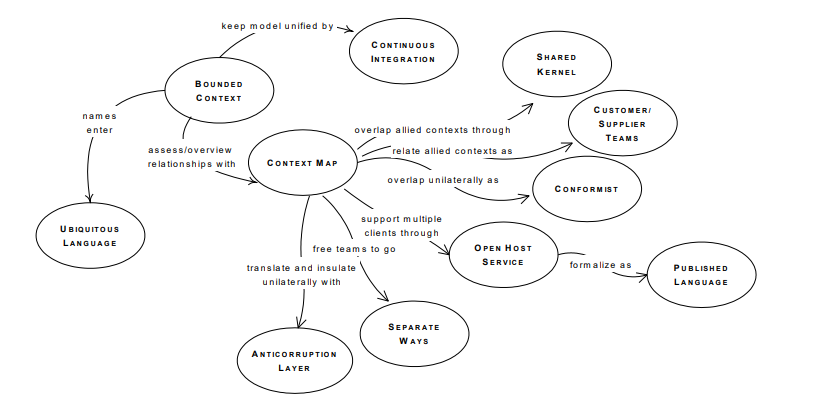
\includegraphics[width = 1\textwidth]{pictures/CacMoHinhChienLuoc/temp.png}

\caption{Sơ đồ về các thành phần trong mô hình chiến lược}

\end{figure}

%!<! - - $ Vẽ lại sau: - - >

%!<! - - $ Vẽ lại sau: - - >

%!<! - - $ Vẽ lại sau: - - >

%!<! - - $ Vẽ lại sau: - - >

%!<! - - $ Vẽ lại sau: - - >

%!<! - - $ Vẽ lại sau: - - >

%!<! - - $ Vẽ lại sau: - - >

%!<! - - $ Vẽ lại sau: - - >

%!<! - - $ Vẽ lại sau: - - >

%!<! - - $ Vẽ lại sau: - - >

%!<! - - $ Vẽ lại sau: - - >

%!<! - - Bối cảnh giới hạn (Bounded Context) - - >

%!<! - - [Giữ cho mô hình thống nhất] Tích hợp Liên tục (Continuous Integration) - - >

%!<! - - [Tính nhất quán trong trao đổi] Ngôn ngữ chung (Ubiquitous Language) - - >

%!<! - - [Tổng quan mối quan hệ] Bản đồ bối cảnh (Context Maps) - - >

%!<! - - Symmetric Relationship: Separate ways, Shared Kernel - - >

%!<! - - Asymmetric Relationship: Customer - Supplier, Conformist, Anti Corruption Layer - - >

%!<! - - - - >

%!<! - - One - to - Many Relationship: Open Host Service, Published Language - - >

%!<! - - dịch và cách ly đơn phương với - - >

%!<! - - [lớp] lớp (Context Maps) - - >

%

%!<! - - "Bản đồ bối cảnh dịch chuyển và cách ly một cách đơn phương để tạo thành cấu trúc lớp." - - >

%!<! - - Tách biệt - - >



% \subsubsection{Bối cảnh giới hạn (Bounded Context)}
% %!<! - - @ - - >

Một miền cần chia đủ nhỏ để phù hợp với một nhóm cụ thể. Để đạt được điều này, chúng ta cần xác định rõ ranh giới giữa các ngữ cảnh.

= > Bối cảnh giới hạn (Bounded Context) giúp định rõ các ranh giới, chia miền thành các phần độc lập để giải quyết sự phức tạp trong mô hình doanh nghiệp.

Bối cảnh giới hạn thể hiện phạm vi kinh doanh của dịch vụ.

![](pictures/BoiCanhGioiHan/___RanhGioi.png)

%!<! - - $VD: - - >
%!<! - - Một vài hướng xác định bối cảnh giới hạn: - - >

Việc xác định bối cảnh giới hạn được điều chỉnh bởi sự gắn kết giữa các miền phụ trong miền kinh doanh.
Dựa vào sơ đồ cấu trúc tổ chức của doanh nghiệp.
Dựa vào modules của các ứng dụng kiến trúc nguyên khối hiện tại (nếu việc phân chia tốt).
Dựa vào trách nhiệm và hoạt động của chuyên gia ngành.

%!<! - - Một số đặc điểm: - - >

Mỗi liên hệ giới hạn phải được thể hiện thông qua một mô hình miền riêng biệt không có sự chia sẻ về mô hình.

%!<! - - $VD: Hình mỗi domain có mô hình riêng... user(id, name) ở domain1, user(id, name, sdt) ở domain2 - - >

Những mô hình được tạo và quản lý độc lập bởi các nhóm.

%!<! - - $VD: - - >

Mô hình miền được xây dựng cho bối cảnh giới hạn chỉ có tác dụng trong phạm vi giới hạn của nó.

%!<! - - $VD: - - >
%!<! - - Hướng dẫn 5/10 - - >

% %!<! - - Bounded Context: https:// thiết kế hướng miền - practitioners.com/home/glossary/bounded - context - - >
% %!<! - - Bounded Context: https:// thiết kế hướng miền - practitioners.com/home/glossary/bounded - context - - >

Trang chủTrang chủBảng chú giảiBối cảnh giới hạn
Bối cảnh giới hạn
Trong thiết kế hướng miền (thiết kế hướng miền), bối cảnh giới hạn là ranh giới xác định phạm vi áp dụng một mô hình nhất định. Nó được sử dụng để tách biệt các mô hình khác nhau và tránh nhầm lẫn. Ý tưởng đằng sau bối cảnh giới hạn là tạo ra các mô hình khác nhau cho các khía cạnh khác nhau của miền và xác định rõ ràng ranh giới giữa chúng, sao cho các thuật ngữ giống nhau có thể được sử dụng với ý nghĩa khác nhau trong các ngữ cảnh khác nhau.

Ví dụ: một khách hàng có thể có nhiều ý nghĩa khác nhau tùy thuộc vào ngữ cảnh: trong ngữ cảnh thanh toán, đó là người nợ tiền; trong bối cảnh vận chuyển, đó là người nhận hàng. Bằng cách tạo một mô hình riêng cho từng ngữ cảnh, chúng ta có thể tránh nhầm lẫn và làm cho mã rõ ràng hơn.

Bối cảnh giới hạn được sử dụng để tạo bản đồ bối cảnh, hiển thị mối quan hệ giữa các mô hình khác nhau và cách chúng tương tác với nhau. Nó cũng giúp xác định các khu vực của miền cần có các mô hình khác nhau và xác định ranh giới giữa chúng.

Bối cảnh giới hạn cũng giúp cải thiện giao tiếp và cộng tác giữa các nhà phát triển, các bên liên quan và chuyên gia ngành bằng cách cung cấp ngôn ngữ chung và hiểu biết chung về miền. Nó cũng thúc đẩy tính mô đun, khả năng bảo trì và khả năng thích ứng của mã.

Khi tạo bối cảnh giới hạn, điều quan trọng là xác định bối cảnh trong đó mô hình được áp dụng, xác định ranh giới của bối cảnh, tạo mô hình phù hợp với mô hình miền tổng thể và truyền đạt bối cảnh tới các bối cảnh khác và miền tổng thể.

% %!<! - - Bounded Context: https:// thiết kế hướng miền - practitioners.com/home/glossary/bounded - context - - >
% %!<! - - Bounded Context: https:// thiết kế hướng miền - practitioners.com/home/glossary/bounded - context - - >
[[Context]] The setting in which a word or statement appears that determines its meaning. See [[Bounded Context]].

Mỗi bounded context nên tương ứng với một nhóm hoặc bộ phận cụ thể trong tổ chức. Sự tương ứng này có thể giúp giảm thiểu sự hiểu lầm và tăng khả năng tương tác giữa các nhóm ngũ.

Ví dụ: khách hàng có thể có nhiều ý nghĩa khác nhau tùy thuộc vào ngữ cảnh: trong ngữ cảnh thanh toán, đó là người nợ tiền; trong bối cảnh vận chuyển, đó là người nhận hàng. Bằng cách tạo một mô hình riêng cho từng ngữ cảnh, chúng ta có thể tránh nhầm lẫn và làm cho mã rõ ràng hơn.

% %!<! - - Bounded Context Relationships : https:// thiết kế hướng miền - practitioners.com/bounded - context - relationship - - >
% %!<! - - Bounded Context Relationships : https:// thiết kế hướng miền - practitioners.com/bounded - context - relationship - - >

Trang chủTrang chủBảng chú giảiBối cảnh giới hạn Mối quan hệ bối cảnh giới hạn
Mối quan hệ bối cảnh giới hạn
Trong Thiết kế hướng miền (thiết kế hướng miền), bối cảnh giới hạn là ranh giới trong đó một mô hình miền cụ thể tồn tại và hợp lệ. Các ngữ cảnh giới hạn giúp xác định phạm vi của mô hình miền và thiết lập sự hiểu biết rõ ràng về ngôn ngữ được sử dụng trong ngữ cảnh đó.

Các bối cảnh giới hạn phải độc lập trong bối cảnh riêng của chúng, nhưng chúng vẫn có thể cần tương tác với các bối cảnh giới hạn khác để hoàn thành trách nhiệm của chính chúng. Mặc dù chúng độc lập về mặt mô hình nhưng chúng có thể cần giao tiếp với các bối cảnh giới hạn khác để trao đổi thông tin hoặc cộng tác trong một số nhiệm vụ nhất định. Vì vậy các bối cảnh giới hạn có thể có mối quan hệ với nhau. Những mối quan hệ này rất quan trọng vì chúng giúp xác định sự tương tác giữa các phần khác nhau của hệ thống, cũng như thiết lập ranh giới và trách nhiệm giữa các nhóm khác nhau làm việc trên cùng một hệ thống. Có một số loại mối quan hệ bối cảnh giới hạn, bao gồm:

Quan hệ đối tác : Đây là mối quan hệ trong đó hai hoặc nhiều bối cảnh giới hạn cộng tác và chia sẻ thông tin. Mối quan hệ hợp tác có thể đạt được thông qua một sự kiện tích hợp hoặc bằng cách gọi một dịch vụ.
Hạt nhân được chia sẻ : Trong mối quan hệ này, hai bối cảnh giới hạn chia sẻ một lược đồ mô hình, mã hoặc CSDL chung. Các thành phần được chia sẻ phải ổn định, hoàn thiện và được cả hai nhóm đồng ý. Những thay đổi được thực hiện đối với các thành phần dùng chung cần phải được phối hợp cẩn thận để đảm bảo chúng không phá vỡ chức năng của bối cảnh khác.
Khách hàng - Nhà cung cấp : Đây là mối quan hệ trong đó một bối cảnh giới hạn cung cấp dịch vụ hoặc dữ liệu cho bối cảnh khác. Bối cảnh khách hàng dựa vào bối cảnh nhà cung cấp để có những khả năng hoặc dữ liệu nhất định. Những thay đổi trong bối cảnh nhà cung cấp có thể tác động đến bối cảnh khách hàng, vì vậy điều quan trọng là phải quản lý mối quan hệ này một cách cẩn thận.
Người theo chủ nghĩa tuân thủ : Mối quan hệ này tồn tại khi một bối cảnh giới hạn tuân theo cùng một ngôn ngữ và khái niệm phổ biến như một bối cảnh giới hạn khác. Điều này đảm bảo rằng giao tiếp giữa hai bối cảnh là rõ ràng và rõ ràng.
Lớp chống đổ vỡ : Đây là mối quan hệ trong đó ngữ cảnh được giới hạn sử dụng một lớp để dịch giữa ngôn ngữ của chính nó và ngôn ngữ của ngữ cảnh giới hạn khác. Điều này cho phép hai ngữ cảnh giao tiếp với nhau ngay cả khi chúng có từ vựng hoặc mô hình khác nhau.
Dịch vụ máy chủ mở : Mối quan hệ này xảy ra khi một bối cảnh giới hạn hiển thị một API công khai, mở mà các ngữ cảnh khác có thể sử dụng. Điều này cho phép các ngữ cảnh khác tận dụng chức năng của ngữ cảnh máy chủ theo cách được tiêu chuẩn hóa.
Ngôn ngữ được xuất bản : Trong mối quan hệ này, một ngữ cảnh giới hạn sẽ xuất bản từ vựng và mô hình của nó cho các ngữ cảnh khác sử dụng. Điều này hữu ích khi nhiều bối cảnh cần cộng tác nhưng không muốn tích hợp trực tiếp. Ngôn ngữ được xuất bản đảm bảo rằng ý nghĩa của các thuật ngữ nhất quán trong mọi ngữ cảnh.
Các cách riêng biệt : Mối quan hệ này đề cập đến tình huống trong đó hai hoặc nhiều bối cảnh giới hạn không còn có mối quan hệ với nhau và các nhóm chịu trách nhiệm về chúng chọn làm việc độc lập.

% %!<! - - Bounded Context Relationships : https:// thiết kế hướng miền - practitioners.com/bounded - context - relationship - - >
% %!<! - - Bounded Context Relationships : https:// thiết kế hướng miền - practitioners.com/bounded - context - relationship - - >

\subsubsection{CI/CD}
%!<! - - @Tích hợp Liên tục (Continuous Integration) - - >

Tích hợp Liên tục (Continuous Integration): là việc các thành viên trong nhóm phát triển tích hợp mã nguồn vào một hệ thống chung thường xuyên. Khi có mã nguồn mới việc tích hợp liên tục sẽ tự động kiểm thử và xây dựng giảm xung đột giữa các phiên bản mã nguồn khác nhau, giúp phát hiện và sửa lỗi sớm hơn.
% CD là gì
% CD là gì
% CD là gì
% CD là gì
% CD là gì
% CD là gì
% CD là gì
% CD là gì
% CD là gì
CI/CD là viết tắt của hai khái niệm quan trọng trong quá trình phát triển phần mềm: Continuous Integration (CI) và Continuous Delivery (CD). Đây là một phương pháp giúp tự động hóa quy trình phát triển, kiểm thử, và triển khai ứng dụng, giúp tăng cường chất lượng phần mềm và giảm thời gian cũng như rủi ro trong quá trình phát triển.

1. **Continuous Integration (CI - Tích hợp liên tục):**
- **Mục tiêu:** Đảm bảo rằng mã nguồn mới được tích hợp vào mã nguồn chính (main codebase) một cách tự động và thường xuyên, giảm thời gian giữa việc viết mã và phát hành.
- **Quy trình:** Mỗi khi một nhà phát triển hoàn thành một tính năng hoặc sửa lỗi, họ tích hợp mã của mình vào mã nguồn chính. Hệ thống CI sẽ tự động kiểm tra mã này bằng cách chạy các bài kiểm thử tự động để đảm bảo rằng nó không làm hỏng hệ thống.

2. **Continuous Delivery (CD - Phân phối liên tục):**
- **Mục tiêu:** Tự động hóa việc triển khai ứng dụng để có thể phân phối bản vá, tính năng hoặc cập nhật một cách nhanh chóng và đáng tin cậy.
- **Quy trình:** Nếu quá trình CI thành công, mã nguồn sẽ được triển khai tự động lên môi trường thử nghiệm (staging environment). Nếu mọi thứ ổn, nó có thể được triển khai tự động lên môi trường sản phẩm (production environment).

3. **Continuous Deployment (CD - Triển khai liên tục):**
- **Khác biệt với Continuous Delivery:** Trong Continuous Deployment, nếu mọi thứ qua bài kiểm thử được tự động và thành công, mã nguồn sẽ tự động triển khai lên môi trường sản phẩm mà không cần sự can thiệp thủ công.
- **Mục tiêu:** Tối ưu hóa quá trình triển khai, giảm thiểu sự chờ đợi và đảm bảo tính ổn định của hệ thống.

4. **Các công cụ thường được sử dụng:**
- **Jenkins, Travis CI, CircleCI:** Đối với CI.
- **Docker, Kubernetes:** Đối với CD, đặc biệt là việc triển khai và quản lý containerized applications.
- **Ansible, Puppet, Chef:** Công cụ tự động hóa cấu hình và triển khai.

Tổng cộng, CI/CD giúp tăng cường khả năng linh hoạt, đảm bảo chất lượng mã nguồn, giảm rủi ro, và giảm thời gian giữa việc phát triển và triển khai sản phẩm.

% CD là gì
% CD là gì
% CD là gì
% CD là gì
% CD là gì
% CD là gì
% CD là gì
% CD là gì
% CD là gì
% CD là gì

Khi một bối cảnh giới hạn đã được xác định, chúng ta cần đảm bảo rằng nó luôn ở trạng thái mới và hoạt động tốt như kỳ vọng. Đáp ứng nhu cầu doanh nghiệp phát triển thay đổi liên tục và nhanh chóng.
Khi cùng vận hành và phát triển xung đột có thể xảy ra ở cùng hoặc khác bối cảnh giới hạn.
= > Vì vậy, cần sử dụng việc tích hợp liên tục tạo ra một quy trình tự động và liên tục từ việc tích hợp mã nguồn, kiểm thử tự động giúp tăng cường chất lượng phần mềm, giảm thời gian và rủi ro trong quá trình phát triển phần mềm.

%!<! - - $VD: jenkins - - >
%!<! - - unit test - - >
%!<! - - test tích hợp - - >

% vở
% thời gian khác nhau

% http://localhost nên không có CD

\subsubsection{Ngôn ngữ chung (Ubiquitous Language)}
%!<! - - @ - - >

Trong quá trình xây dựng mô hình miền, cần có đối thoại trao đổi giữa những người thiết kế phần mềm và chuyên gia ngành để hiểu đúng về miền. Tuy nhiên, nhóm kinh doanh sử dụng ngôn ngữ kinh doanh và nhóm công nghệ có xu hướng sử dụng các thuật ngữ kỹ thuật trong giao tiếp của họ. Người phát triển phần mềm tập trung vào lớp, phương thức, thuật toán, trong khi chuyên gia ngành thường sử dụng ngôn ngữ chuyên ngành của họ. Sự khác biệt về ngôn ngữ giữa các thành viên có thể dẫn đến những thách thức về giao tiếp.

Trong các lĩnh vực kinh doanh khác nhau, một thuật ngữ có thể được sử dụng trong nhiều miền, cùng với ý nghĩa khác nhau gây ra sự nhầm lẫn và hiểu sai cho các người phát triển phần mềm cũng như các chuyên gia ngành.

%!<! - - = > Thiết kế hướng miền đề xuất sử dụng ngôn ngữ chung để giải quyết những thách thức ngôn ngữ. - - >

Ngôn ngữ chung (Ubiquitous Language) là một trong những mô hình chiến lược của thiết kế hướng miền, thiết lập một ngôn ngữ chung trong từng bối cảnh kinh doanh.
Ngôn ngữ chung được xác định bởi từ vựng và có định nghĩa rõ ràng về ngữ cảnh từ vựng áp dụng.

%!<! - - Một số đặc điểm: - - >

Ngôn ngữ chung được sử dụng bởi cả chuyên gia ngành và chuyên gia công nghệ.
Có nhiều ngôn ngữ chung trong một tổ chức được mỗi nhóm tạo và quản lý một cách độc lập.
Việc tạo ra ngôn ngữ chung là một quá trình liên tục. Ngôn ngữ chung phát triển theo thời gian thông qua sự cộng tác giữa doanh nghiệp và các chuyên gia công nghệ.

Các thành viên phải sử dụng ngôn ngữ chung cho công việc và trong toàn bộ hệ thống như:

Sử dụng trong cuộc thảo luận trao đổi giữa các chuyên gia ngành và các chuyên gia công nghệ
Sử dụng trong các tài liệu phát triển của nhóm
Sử dụng trong sản phẩm và kiểm thử phần mềm

![](pictures/NgonNguChung/___NgonNguPhoBien.png)

%!<! - - $VD: Ngôn ngữ chung được sử dụng, áp dụng trong toàn bộ hệ thống. - - >
%!<! - - Hướng dẫn 5/7 - - >

%!<! - - [[Ubiquitous Language]] A language structured around the domain model and used by all team members to connect all the activities of the team with the software. - - >
% %!<! - - Ubiquitous Language : https:// thiết kế hướng miền - practitioners.com/home/glossary/ubiquitous - language - - >
% %!<! - - Ubiquitous Language : https:// thiết kế hướng miền - practitioners.com/home/glossary/ubiquitous - language - - >
% %!<! - - Ubiquitous Language : https:// thiết kế hướng miền - practitioners.com/home/glossary/ubiquitous - language - - >
% %!<! - - Ubiquitous Language : https:// thiết kế hướng miền - practitioners.com/home/glossary/ubiquitous - language - - >
% %!<! - - Ubiquitous Language : https:// thiết kế hướng miền - practitioners.com/home/glossary/ubiquitous - language - - >
% %!<! - - Ubiquitous Language : https:// thiết kế hướng miền - practitioners.com/home/glossary/ubiquitous - language - - >
% %!<! - - Ubiquitous Language : https:// thiết kế hướng miền - practitioners.com/home/glossary/ubiquitous - language - - >

Trang chủTrang chủBảng chú giải ngôn ngữ chung
ngôn ngữ chung
Trong thiết kế hướng miền (thiết kế hướng miền), ngôn ngữ chung là ngôn ngữ dùng chung được sử dụng để mô tả miền và mô hình miền. Đó là ngôn ngữ chung được các nhà phát triển, các bên liên quan và chuyên gia ngành sử dụng để giao tiếp và hiểu miền kinh doanh.

Ý tưởng đằng sau ngôn ngữ chung là tạo ra sự hiểu biết chung về miền bằng cách sử dụng một ngôn ngữ chung để mô tả các khái niệm và mối quan hệ trong miền. Ngôn ngữ chung này nên được sử dụng nhất quán trong suốt quá trình phát triển phần mềm, từ giai đoạn phân tích và thiết kế đến giai đoạn triển khai và bảo trì.

ngôn ngữ chung phải dựa trên ngôn ngữ đã được sử dụng trong miền và nên được sử dụng để đặt tên cho các lớp, giao diện, phương thức và biến trong mã. Điều này giúp đảm bảo rằng mã có tính biểu cảm, dễ hiểu và phù hợp với nhu cầu kinh doanh.

Mục tiêu của ngôn ngữ chung là đảm bảo rằng phần mềm phù hợp với nhu cầu kinh doanh và miền kinh doanh được thể hiện chính xác trong phần mềm. Nó cũng giúp cải thiện khả năng giao tiếp và cộng tác giữa các nhóm khác nhau và đảm bảo rằng phần mềm có thể bảo trì và thích ứng với sự thay đổi.

Điều quan trọng cần lưu ý là ngôn ngữ chung không chỉ giới hạn ở cách đặt tên mã mà còn là một cách để đảm bảo rằng các khái niệm và mối quan hệ kinh doanh được thể hiện chính xác trong phần mềm và phần mềm phù hợp với nhu cầu kinh doanh.

Dưới đây là một số ví dụ về cách áp dụng ngôn ngữ chung trong thiết kế hướng miền:

Quy ước đặt tên : Tên của các lớp, giao diện, phương thức và biến trong mã phải dựa trên ngôn ngữ đã được sử dụng trong miền. Ví dụ: trong miền thương mại điện tử, khái niệm “đặt hàng” phải được gọi một cách nhất quán là “đặt hàng” trong toàn bộ mã, thay vì sử dụng các tên khác nhau như “mua hàng” hoặc “giao dịch”.
Mô hình hóa quy trình nghiệp vụ : Các quy trình nghiệp vụ trong miền phải được mô hình hóa bằng cách sử dụng cùng các thuật ngữ và khái niệm đã được sử dụng trong miền. Ví dụ: trong lĩnh vực chăm sóc sức khỏe, quy trình “tiếp nhận bệnh nhân” phải được đề cập đến việc sử dụng các thuật ngữ và khái niệm tương tự được các chuyên gia chăm sóc sức khỏe sử dụng, chẳng hạn như “quy trình tiếp nhận” hoặc “quy trình đăng ký bệnh nhân”
Mô hình hóa các thực thể kinh doanh : Các thực thể kinh doanh trong miền phải được mô hình hóa bằng cách sử dụng cùng các thuật ngữ và khái niệm đã được sử dụng trong miền. Ví dụ: trong lĩnh vực tài chính, khái niệm “tài khoản” phải được gọi một cách nhất quán là “tài khoản” trong toàn bộ mã, thay vì sử dụng các tên khác nhau như “sổ cái” hoặc “hồ sơ tài chính”
Giao tiếp : ngôn ngữ chung nên được sử dụng trong mọi giao tiếp, bao gồm các cuộc họp, tài liệu và nhận xét mã, để đảm bảo rằng mọi người đều sử dụng các thuật ngữ và khái niệm giống nhau.

% %!<! - - Ubiquitous Language : https:// thiết kế hướng miền - practitioners.com/home/glossary/ubiquitous - language - - >
% %!<! - - Ubiquitous Language : https:// thiết kế hướng miền - practitioners.com/home/glossary/ubiquitous - language - - >
% %!<! - - Ubiquitous Language : https:// thiết kế hướng miền - practitioners.com/home/glossary/ubiquitous - language - - >
% %!<! - - Ubiquitous Language : https:// thiết kế hướng miền - practitioners.com/home/glossary/ubiquitous - language - - >

%!<! - - Bằng cách sử dụng ngôn ngữ chung như trên, chúng ta có thể tạo ra một mô hình thiết kế hướng miền rõ ràng và dễ hiểu, giúp các nhóm phát triển, quản lý dự án và người dùng hiểu rõ về các yêu cầu và chức năng của hệ thống. - - >

\subsubsection{Bản đồ bối cảnh (Context Maps)}
\newpage
\begin{center}
{\bfseries NHẬN XÉT CỦA GIẢNG VIÊN HƯỚNG DẪN}
\end{center}
1.	Mục đích và nội dung của đồ án:

\vspace{4ex} % Thêm khoảng cách dọc

2.	Kết quả đạt được:

3.	Ý thức làm việc của sinh viên:

Hà Nội, \today

\textbf{Giảng viên hướng dẫn}

\textit{(Ký và ghi rõ họ tên)}

\newpage


% \subsection{Các mẫu kỹ thuật (Tactical Patterns)}
% %!<! - - Tactical Design : https:// thiết kế hướng miền - practitioners.com/?page_id = 453 - - >

Trang chủTrang chủBảng chú giảiThiết kế hướng miền Thiết kế chiến thuật

Thiết kế chiến thuật

Trong thiết kế hướng miền, thiết kế chiến thuật đề cập đến quá trình thiết kế các thành phần riêng lẻ của hệ thống phần mềm để triển khai mô hình miền. Nó liên quan đến việc chia mô hình miền thành các đơn vị chức năng nhỏ hơn, gắn kết và liên kết lỏng lẻo được gọi là bối cảnh giới hạn, tập hợp, thực thể, đối tượng giá trị và dịch vụ miền. Thiết kế chiến thuật liên quan đến việc thiết kế các đơn vị này và mối quan hệ giữa chúng. Nó cũng liên quan đến việc lựa chọn các mẫu, chiến lược và chiến thuật phù hợp để đạt được mục tiêu thiết kế trong khi vẫn tuân thủ các nguyên tắc thiết kế hướng miền.

Các yếu tố của thiết kế chiến thuật trong Thiết kế hướng miền (thiết kế hướng miền) như sau:

Ngữ cảnh giới hạn : Ngữ cảnh giới hạn xác định ranh giới rõ ràng xung quanh một phần cụ thể của mô hình miền và ngôn ngữ chung đi kèm với nó.

Tập hợp : Tập hợp là các cụm đối tượng liên quan được coi là một đơn vị công việc duy nhất.

Thực thể : Thực thể là các đối tượng có danh tính và vòng đời duy nhất và có thể thay đổi theo thời gian.

Đối tượng giá trị : Đối tượng giá trị là các đối tượng không có danh tính duy nhất nhưng được xác định bởi các thuộc tính của chúng.

Dịch vụ : Dịch vụ là các hoạt động hoặc hành vi không phù hợp một cách tự nhiên trong một thực thể hoặc đối tượng giá trị.

Sự kiện miền : Sự kiện miền là những sự kiện quan trọng xảy ra trong miền mà các phần khác của hệ thống có thể cần biết.

Dịch vụ miền : Dịch vụ miền là các hoạt động hoặc hành vi áp dụng cho toàn bộ miền thay vì cho một thực thể hoặc đối tượng giá trị cụ thể.

Nhà máy : Nhà máy được sử dụng để tạo các đối tượng hoặc tập hợp phức tạp có thể yêu cầu nhiều bước hoặc logic phức tạp.

Kho lưu trữ : Kho lưu trữ được sử dụng để trừu tượng hóa việc lưu trữ và truy xuất các tập hợp và thực thể.

Thiết kế chiến thuật được gọi như vậy vì nó tập trung vào các quyết định chiến thuật liên quan đến mô hình hóa miền và triển khai logic nghiệp vụ trong mã. Thiết kế chiến thuật là quá trình triển khai các mẫu, nguyên tắc và thực tiễn thiết kế hướng miền để tạo ra một hệ thống phần mềm linh hoạt, có thể bảo trì và có thể mở rộng. Đây là một phần thiết yếu của thiết kế hướng miền giúp các nhà phát triển sắp xếp mã của họ và cải thiện chất lượng của hệ thống phần mềm. Thiết kế chiến thuật cung cấp một bộ nguyên tắc và phương pháp hay nhất mà nhà phát triển có thể làm theo để tạo mô hình miền phù hợp với yêu cầu kinh doanh và có thể phát triển theo thời gian.

%!<! - - $ Vẽ lại sau: - - >

%!<! - - $ Vẽ lại sau: - - >

%!<! - - $ Vẽ lại sau: - - >

%!<! - - $ Vẽ lại sau: - - >

%!<! - - $ Vẽ lại sau: - - >

%!<! - - $ Vẽ lại sau: - - >

%!<! - - $ Vẽ lại sau: - - >

%!<! - - $ Vẽ lại sau: - - >

%!<! - - $ Vẽ lại sau: - - >

%!<! - - $ Vẽ lại sau: - - >

%!<! - - $ Vẽ lại sau: - - >

%!<! - - $ Vẽ lại sau: - - >

%!<! - - $ Vẽ lại sau: - - >

% \subsubsection{xxxxxxx}
% \newpage
\begin{center}
{\bfseries NHẬN XÉT CỦA GIẢNG VIÊN HƯỚNG DẪN}
\end{center}
1.	Mục đích và nội dung của đồ án:

\vspace{4ex} % Thêm khoảng cách dọc

2.	Kết quả đạt được:

3.	Ý thức làm việc của sinh viên:

Hà Nội, \today

\textbf{Giảng viên hướng dẫn}

\textit{(Ký và ghi rõ họ tên)}

\newpage


% %
% Yêu cầu nghiệp vụ của từng sub
% %
% Sơ đồ if else Đ S
% %
% sub trước model
% %
%%%%%%%%%%%%%%%%%%%%%%%%%%%%%%%%%%%%%
\end{document}

\section{xxxxxxx}
\subsection{xxxxxxx}
\subsubsection{xxxxxxx}
\newpage
\begin{center}
{\bfseries NHẬN XÉT CỦA GIẢNG VIÊN HƯỚNG DẪN}
\end{center}
1.	Mục đích và nội dung của đồ án:

\vspace{4ex} % Thêm khoảng cách dọc

2.	Kết quả đạt được:

3.	Ý thức làm việc của sinh viên:

Hà Nội, \today

\textbf{Giảng viên hướng dẫn}

\textit{(Ký và ghi rõ họ tên)}

\newpage


% phải có CQRS (Phân chia trách nhiệm truy vấn lệnh)

CQRS là một mẫu kiến trúc riêng biệt có thể được sử dụng kết hợp với thiết kế hướng miền để đạt được những lợi ích nhất định, chẳng hạn như cải thiện hiệu suất và khả năng mở rộng. Tuy nhiên, nó không phải là một yêu cầu để triển khai thiết kế hướng miền.

% phải có event
Ngôn ngữ chung (Ubiquitous Language)

%%%%%%%%%%%%%%%%%%%%%%%%%%%%%%%%%%%%%
\end{document} % kết thúc